\date{}
\title{}
\date{}
\usepackage[outputdir=latex.out]{minted}
\begin{document}
\begin{frame}
    \titlepage
\end{frame}


\makeatletter
\newenvironment<>{btHighlight}[1][]
{\begin{onlyenv}#2\begingroup\tikzset{bt@Highlight@par/.style={#1}}\begin{lrbox}{\@tempboxa}}
{\end{lrbox}\bt@HL@box[bt@Highlight@par]{\@tempboxa}\endgroup\end{onlyenv}}

\newcommand<>\btHL[1][]{%
  \only#2{\begin{btHighlight}[#1]\bgroup\aftergroup\bt@HL@endenv}%
}
\def\bt@HL@endenv{%
  \end{btHighlight}%   
  \egroup %
}
\tikzset{
    btHLbox/.style={
        fill=red!30,outer sep=0pt,inner xsep=1pt, inner ysep=0pt, rounded corners=3pt
    },
}
\newcommand{\bt@HL@box}[2][]{%
  \tikz[#1]{%
    \pgfpathrectangle{\pgfpoint{1pt}{0pt}}{\pgfpoint{\wd #2}{\ht #2}}%
    \pgfusepath{use as bounding box}%
    \node[text width={},draw=none,anchor=base west, btHLbox, minimum height=\ht\strutbox+1pt,#1]{\raisebox{1pt}{\strut}\strut\usebox{#2}};
  }%
}

\lst@CCPutMacro
    \lst@ProcessOther {"2A}{%
      \lst@ttfamily 
         {\raisebox{2pt}{*}}% used with ttfamily
         {\raisebox{2pt}{*}}}% used with other fonts
    \@empty\z@\@empty

\lstdefinelanguage
   [x8664gas]{Assembler}     % add a "x64" dialect of Assembler
   [x86masm]{Assembler} % based on the "x86masm" dialect
   % with these extra keywords:
   {morekeywords={CDQE,CQO,CMPSQ,CMPXCHG16B,JRCXZ,LODSQ,MOVSXD,%
                  POPFQ,PUSHFQ,SCASQ,STOSQ,IRETQ,RDTSCP,SWAPGS,.TEXT,.STRING,.ASCIZ,%
                  BEQ,LW,SW,LB,SB,ADDIU,J,BEQZ,BNEZ,BNE,%
                  MOVUPD,MULPD,MOVSD,MULSD,%
                  SHLADD,MOV,CMP.LT,TBIT.NZ,BR.RET.SPTK.MANY,%
                  ADDQ,POPQ,PUSHQ,RRMOVQ,MRMOVQ,RMMOVQ,IRMOVQ,%
                  <-,LL,SC,ADDI,ADDL,VMOVDQA,ADDQ,CMPL,JB,JBE,MOVL,CLTQ,%
                  MOVW,PUSHW,MOV,ADD,SUB,INT,PUSH,MOV,ADD,REP,MOVSB,%
                  TESTQ,CMPQ,MOVL,MOVQ,ADDQ,JMPQ,XORQ,%
                  LEAQ,LEAL,LEA,RETQ,RET,POPL,POPW,PUSHL,PUSHW,%
                  LEAW,%
                  SUBQ,SYSCALL,.ASCII,CALLQ,MOVSLQ,JMP,ANDQ,SHRQ,MOVB,INCQ,TESTL,XORL,%
                  SHRL,LEAL,SARL,SUBL,IMULL,IMULQ,MOVDQU,PADDD,XORL,%
                  MOVZBL,MOVZB,SHRB,SRAL,SHRL,ANDL,%
                  CMOVNS,SRAL,SRAQ,MOVZBW,MOVZBQ,%
                  PADDW,PADDQ,MODUPS,MOVAPD,%
                  MOVL,RET,.GLOBL,%
		  PAUSE,LFENCE,JMP,%
                  },
    deletekeywords={eax,ebx,sp,si,cx,di,ds,cs,es,fs,dx,ax,bx,al,esi,ebp,ecx,rip,eip,edx,edi,rdi,esp},
    deletekeywords=[2]{size},
    alsoletter={\%},
    alsoother={()},
    emphstyle={\color{violet!50!black}},
    emph={\%rax,\%rbx,\%rcx,\%rdx,\%r8,\%r9,\%r10,\%r11,\%r12,\%r13,\%r14,\%r15,\%eax,\%ebx,\%sp,\%si,\%cx,\%di,\%ds,\%cs,\%es,\%fs,\%dx,\%ax,\%bx,\%al,\%esi,\%ebp,\%ecx,\%rip,\%eip,\%edx,\%edi,\%rdi,\%esp,\%rsp},
    %moreemph={eax,ebx,sp,si,cx,di,ds,cs,es,fs,dx,ax,bx,al,esi,ebp,ecx,rip,eip,edx,edi,rdi,esp},
    morecomment=[l]{\#},
    morecomment=[l]{\/\/},
    morecomment=[s]{/*}{*/},
    sensitive=false,
    keepspaces=true} % et

\lstalias[]{myasm}[x8664gas]{Assembler}

\lstdefinelanguage{JavaScript}{
  keywords={typeof, new, true, false, catch, function, return, null, catch, switch, var, if, in, while, do, else, case, break},
  ndkeywords={class, export, boolean, throw, implements, import, this},
  sensitive=false,
  comment=[l]{//},
  morecomment=[s]{/*}{*/},
  morestring=[b]',
  morestring=[b]"
}

\newcommand{\keywordstyle}{\sourcecodeprolight\bfseries\color{blue!30!black}}
\newcommand{\stringstyle}{\color{blue!20!black}\ttfamily}

\lstset{
    language=C,
    basicstyle=\sourcecodepro\EmptyMapping,
    escapechar=`,
    keywordstyle=\keywordstyle\EmptyMapping,
    identifierstyle=\sourcecodepro\EmptyMapping,
    numberstyle=\small\color{black!70},
    commentstyle=\color{red!60!black}\ttfamily\itshape,
    stringstyle=\color{blue!20!black}\ttfamily,
    ndkeywordstyle=\bfseries\color{blue!30!black},
    upquote=true,
}



\lstdefinestyle{medium}{
    basicstyle=\sourcecodepro\EmptyMapping\fontsize{12}{13}\selectfont,
    keywordstyle=\sourcecodepro\EmptyMapping\fontsize{12}{13}\selectfont\keywordstyle,
}

\lstdefinestyle{small}{
    basicstyle=\sourcecodepro\EmptyMapping\small,
    keywordstyle=\sourcecodepro\EmptyMapping\small\keywordstyle,
}

\lstdefinestyle{smaller}{
    basicstyle=\sourcecodepro\EmptyMapping\fontsize{11}{12}\selectfont,
    keywordstyle=\sourcecodepro\EmptyMapping\fontsize{11}{12}\selectfont\keywordstyle,
}

\lstdefinestyle{size105}{
    basicstyle=\sourcecodepro\EmptyMapping\fontsize{10.5}{11.5}\selectfont,
    keywordstyle=\sourcecodepro\EmptyMapping\fontsize{10.5}{11.5}\selectfont\keywordstyle,
}

\lstdefinestyle{size10}{
    basicstyle=\sourcecodepro\EmptyMapping\fontsize{10}{11}\selectfont,
    keywordstyle=\sourcecodepro\EmptyMapping\fontsize{10}{11}\selectfont\keywordstyle,
}

\lstdefinestyle{size9}{
    basicstyle=\sourcecodepro\EmptyMapping\fontsize{9}{10}\selectfont,
    keywordstyle=\sourcecodepro\EmptyMapping\fontsize{9}{10}\selectfont\keywordstyle,
}
\lstdefinestyle{size8}{
    basicstyle=\sourcecodepro\EmptyMapping\fontsize{8}{9}\selectfont,
    keywordstyle=\sourcecodepro\EmptyMapping\fontsize{8}{9}\selectfont\keywordstyle,
}



\lstdefinestyle{script}{
    basicstyle=\sourcecodepro\EmptyMapping\scriptsize,
    keywordstyle=\sourcecodepro\EmptyMapping\scriptsize\bfseries,
}




\begin{frame}{last time}
    \begin{itemize}
    \item using use-after-free exploits
        \begin{itemize}
        \item ``toolbox'' of two objects in same place in memory
        \item info leak from pointer in same place as readable values
        \item code exec from VTable and data at same place
        \end{itemize}
    \item Chrome exploit example:
        \begin{itemize}
        \item multiple objects
        \item triggering exploit multiple times with JavaScript
        \end{itemize}
    \item integer overflow
    \end{itemize}
\end{frame}

\begin{frame}{quiz Q1}
    \begin{itemize}
    \item global offset table with RELRO
    \vspace{.5cm}
    \item global offset table region loaded as writeable
    \item then fill in addresses based on loaded libraries
        \begin{itemize}
        \item even if not randomized, not determined until after program starts
        \item \ldots so can't be loaded read-only
        \end{itemize}
    \item then change permissions
    \end{itemize}
\end{frame}
\begin{frame}[fragile]{quiz Q4}
\begin{Verbatim}[fontsize=\fontsize{10}{11}]
(e.function /* X */)(input2 /* Y */, input3 /* Z */);
\end{Verbatim}
\hrule
effect of code in vulernable:
\begin{Verbatim}[fontsize=\fontsize{10}{11}]
    mov $Y, %rdi
    mov $Z, %rsi
    call X // push $AFTER_CALL; jmp X
AFTER_CALL:
\end{Verbatim}
\begin{itemize}
\item goal: set \%rsp to ROP chain, then run ret
\item 0x4050d9: popq \%rsp, ret
    \begin{itemize}
    \item if X = 0x4050d9, sets stack pointer to AFTER\_CALL
    \item BUT if we can run it with ROP chain address pushed already
    \item will reset stack pointer to its value
    \end{itemize}
\item 0x413eb6: pushq \%rsi; orw \%bh, \%bh; jmp *\%rdi
    \begin{itemize}
    \item if X = 0x413eb6:
    \item push RSI (Z) to stack --- ideal setup for 0x4050d9
    \item jump to RDI (Y)
    \end{itemize}
\end{itemize}
\end{frame}



\section{integer overflow}
\begin{frame}{bounds-checking?}
    \begin{itemize}
    \item so far: mistake is no bounds checking
    \item run input function without telling it how much space
    \vspace{.5cm}
    \item so, we avoid this by checking sizes, right?
    \item common problem: bugs in size checking code
    \item integer overflow (or underflow)
    \end{itemize}
\end{frame}



\begin{frame}[fragile,label=intOverflowEx]{integer overflow example (1)}
\lstset{
    language=C,
    morekeywords=item,
    style=smaller,
    moredelim={**[is][\btHL<2|handout:0>]{~2~}{~end~}},
}
\begin{tikzpicture}
\node[anchor=north east] (code) at (-1,0) {
\begin{lstlisting}
item *load_items(int len) {
  int total_size = ~2~len * sizeof(item);~end~
  if (total_size >= LIMIT) {
    return NULL;
  }
  item *items = malloc(total_size);
  for (int i = 0; i < len; ++i) {
    int failed = read_item(&items[i]);
    if (failed) {
      free(items);
      return NULL;
    }
  }
  return items;
}
\end{lstlisting}
};
\node[align=left,anchor=north west,font=\small] (t1) at (0,0) {
    {\tt len} = {\tt 0x4000 0001} \\
    {\tt sizeof(item)} = {\tt 0x10}
};
\node[align=left,anchor=north west,font=\small] (t2) at (t1.south west) {
    {\tt total\_size} = \\
    {\tt 0x\textcolor{red}{4} 0000 0010} \\
};
\end{tikzpicture}
\end{frame}

\begin{frame}[fragile,label=intOverflowEx]{integer overflow example (2)}
\lstset{
    language=C,
    morekeywords=item,
    style=smaller,
    moredelim={**[is][\btHL<2|handout:0>]{~2~}{~end~}},
}
\begin{tikzpicture}
\node[anchor=north east] (code) at (-1,0) {
\begin{lstlisting}
/* adapted from https://project-zero.issues.chromium.org/issues/42451651 
   Windows Kernel bug! */
char *FormatNumber(char *source, short source_len) {
    unsigned short dest_size = source_len * 6;
    char *dest = malloc(dest_size);
    char *p = dest;
    for (unsigned short i = 0; < source_len; i += 1) {
        *p++ = "0123456789ABCDEF"[*source >> 4];
        *p++ = "0123456789ABCDEF"[*source & 0xF];
        *p++ = ' ';
        source++;
    }
}

\end{lstlisting}
};
\node[align=left,anchor=north west,font=\small] (t1) at (0,0) {
    {\tt source\_len} = {0x2AAB} \\
    {\tt sizeof(item)} = {\tt 0x{\color{red}1}0002}
};
\end{tikzpicture}
\end{frame}

 % split

\usetikzlibrary{calc}

\begin{frame}[fragile,label=intUOEx]{integer under/overflow: real example}
    \begin{itemize}
        \item part of another Google Chrome exploit by Pinkie Pie:
    \end{itemize}
    \begin{lstlisting}[language=C,style=small,morekeywords={uint32,size_t}]
// In graphics command processing code:
uint32 ComputeMaxResults(size_t size_of_buffer) {
    return (size_of_buffer - sizeof(uint32)) / sizeof(T);
} 
size_t ComputeSize(size_t num_results) {
    return sizeof(T) * num_results + sizeof(uint32);
} 
// exploit: size_of_buffer < sizeof(uint32)
\end{lstlisting}
    \begin{itemize}
        \item result: write 8 bytes after buffer 
            \begin{itemize}
                \item sometimes overwrites data pointer
            \end{itemize}
    \end{itemize}
\imagecredit{via \url{https://blog.chromium.org/2012/05/tale-of-two-pwnies-part-1.html}}
\end{frame}



\subsection{exercise}
\begin{frame}[fragile,label=intOverflowEx]{exercise}
\lstset{
    language=C,
    morekeywords=item,
    style=smaller,
    moredelim={**[is][\btHL<2|handout:0>]{~2~}{~end~}},
}
\begin{tikzpicture}
\node[anchor=north east] (code) at (-1,0) {
\begin{lstlisting}
void vulnerable() {
  int items[100];
  int count;
  bool success = try_read_input(&count);
  if (!success) { ... }
  if (count * sizeof() >= sizeof(items)) {
    printf("cannot handle that many\n"); return;
  }
  for (int i = 0; i < count; i += 1) {
      if (!try_read_input(&items[i])) { 
        printf("preature end of input\n"); return;
      }
  }
  process_items(items);
}
\end{lstlisting}
};
\end{tikzpicture}
assume return address immediately after items array: \\
Q: what first input number to provide? \\
Q: how to encode return address replacement 0x12345678 ?
\end{frame}



\subsection{avoiding overflow}
% FIXME
\begin{frame}{techniques for avoiding?}
\end{frame}
\subsection{trapping on overflow}
% FIXME \begin{frame}{overflow and undefined behavior}
\begin{itemize}
\item C standard: some things are \textit{undefined behavior}
\item C compiler can do anything in those cases
\vspace{.5cm}
\item \textit{signed integer overflow} is undefined
\item \textit{unsigned integer overflow} must wrap around
\end{itemize}
\end{frame}

\begin{frame}[fragile]{-fsanitize=undefined}
\begin{Verbatim}[fontsize=\small]
int x = INT_MAX -1; int y = 5; printf("%d\n", x * y);
\end{Verbatim}
\begin{itemize}
\item compile with \texttt{-fsanitize=undefined}:
    \begin{itemize}
        \item \texttt{test.c:...: runtime error: signed integer overflow: 2147483646 * 5 cannot be represented in type 'int}
    \end{itemize}
\item compile with \texttt{-ftrapv}: \texttt{Aborted (core dumped)}
\end{itemize}
\begin{Verbatim}[fontsize=\small]
unsigned x = INT_MAX -1; unsigned y = 5; printf("%u\n", x * y);
\end{Verbatim}
\begin{itemize}
\item compile with \texttt{-fsanitize=undefined} or \texttt{-ftrapv}: NO ERROR
\end{itemize}
\end{frame}

\begin{frame}[fragile]{in Rust (1)}
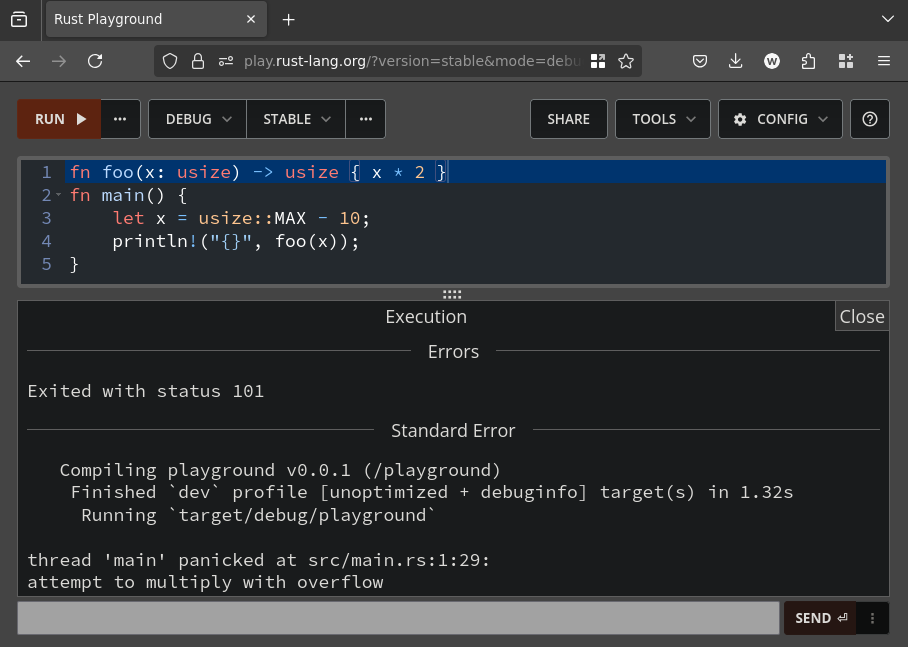
\includegraphics[height=0.9\textheight]{../overflow-int/rust-oflow-trap}
\end{frame}

\begin{frame}[fragile]{in Rust (2)}
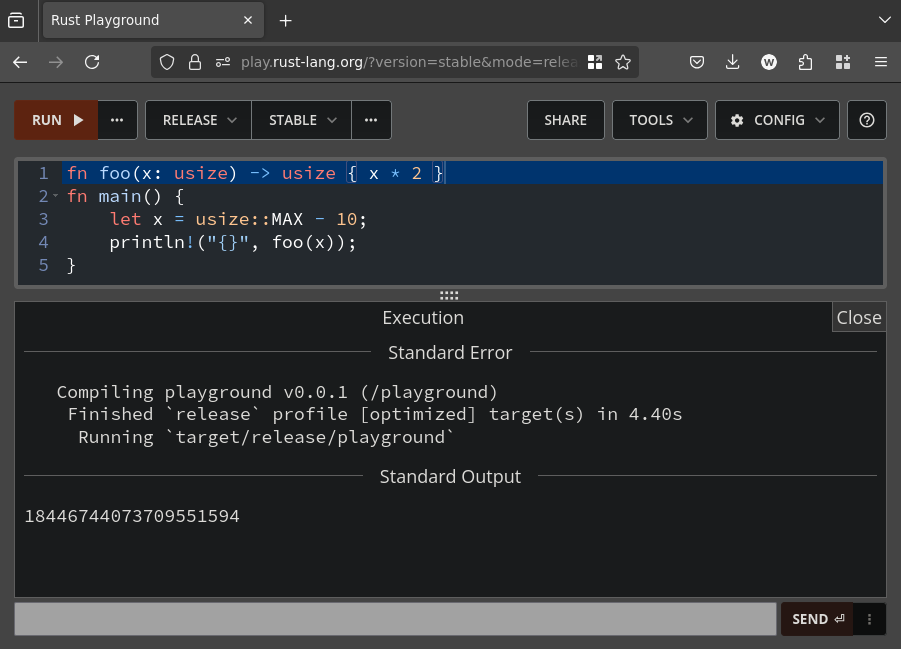
\includegraphics[height=0.9\textheight]{../overflow-int/rust-oflow-notrap}
\end{frame}

\begin{frame}[fragile]{in Rust (3)}
\begin{Verbatim}[fontsize=\fontsize{11}{12}]
let x = usize::MAX - 10; let y = 10usize;
println!("{} {}", x.saturating_mul(2), y.saturating_mul(2));
// 18446744073709551615 20
    // 18446744073709551615==usize::MAX
println!("{:?} {:?}", x.checked_mul(2), y.checked_mul(2));
// None Some(30)
println!("{} {}", x.wrapping_mul(2), y.wrapping_mul(2));
// 18446744073709551594 20
    // 18446744073709551594==usize::MAX-21
\end{Verbatim}
\end{frame}


\begin{frame}{compiler support to avoid?}
    \begin{itemize}
    \item GCC/Clang options:
        \begin{itemize}
        \item -fsanitize=undefined
        \item -ftrapv
        \end{itemize}
    \item better programming language design:
        \begin{itemize}
        \item Rust, \ldots
        \end{itemize}
    \end{itemize}
\end{frame}

% FIXME: examples of -fsanitize=undefined, -ftrapv
% FIXME: wrapping behavior in C for usnignedj
% FIXME: example in Rust + other int operators

\begin{frame}{overflow, C and undefined behavior}
\end{frame}




\section{Rust}

% FIXME
\subsection{aside: why do people like C/C++?}
\begin{frame}{why are people still using C/C++?}
    \begin{itemize}
    \item Python, Java, \ldots are great languages
    \item why are people using C, C++, etc.?
        \begin{itemize}
        \item which seem horrible for security?
        \end{itemize}
    \vspace{.5cm}
    \item history + good support
        \begin{itemize}
        \item lots of libraries in C, C++, \ldots
        \end{itemize}
    \item \myemph<2>{``zero overhead''}
        \begin{itemize}
        \item safe languages don't make it easy to get ``close to the machine''
        \item e.g. garbage collection overhead
        \item e.g. array checking overhead
        \end{itemize}
    \item no language VM --- easier to distribute
    \end{itemize}
\end{frame}

% FIXME

\subsection{safety + escape hatch}
\begin{frame}{safety rules + escape hatch}
    \begin{itemize}
    \item idea: can avoid out-of-bounds, etc. with safety rules
    \item \ldots but safety rules don't allow us to do some things fast
    \vspace{.5cm}
    \item so: have ``escape hatch'' to avoid safety checks in those cases
    \item hope: code that uses escape hatch can be tightly checked
        \begin{itemize}
        \item good target for expensive program analysis
        \end{itemize}
    \end{itemize}
\end{frame}



\begin{frame}[fragile,label=javaEscapeHatch]{Java: unofficial escape hatch}
    \begin{itemize}
    \item Oracle JDK and OpenJDK come with a class called \texttt{com.sun.Unsafe}
    \item Example methods:
    \end{itemize}
\begin{lstlisting}
public long allocateMemory(long size);
                        // returns pointer value
public void freeMemory(long address);
public long getLong(long address);
public void putLong(long address, long x);
\end{lstlisting}
    \begin{itemize}
    \item can be used to, e.g.,  write ``fast'' IntArray class
    \end{itemize}
\end{frame}


\begin{frame}{so, if Java has escape hatch\ldots}
    \begin{itemize}
    \item why do people not want to write \\ their performance-sensitive programs in Java?
    \vspace{.5cm}
    \item hard to integrate code that uses escape hatch with normal Java code
    \item hard to efficiently avoid dangling pointers when using escape hatch
        \begin{itemize}
        \item Is it safe to freeMemory from my FastIntArray class?
        \end{itemize}
    \item slow to pass garbage collected references to/from C/assembly code
    \item hard to avoid using garbage collector
        \begin{itemize}
        \item garbage collector performance can be variable
        \end{itemize}
    \end{itemize}
\end{frame}


\subsection{general philosophy}

\begin{frame}{Rust philosophy}
    \begin{itemize}
    \item default rules that only allow `safe' things
        \begin{itemize}
        \item no dangling pointers
        \item no out-of-bounds accesses
        \end{itemize}
    \item escape hatch to use ``raw'' pointers or unchecked libraries
    \item escape hatch can be used to write useful libraries
        \begin{itemize}
            \item e.g. Vector/ArrayList equivalent
            \item \myemph{expose interface that is safe}
        \end{itemize}
    \end{itemize}
\end{frame}



\subsection{general syntax (1)}
\usetikzlibrary{positioning,shapes.callouts}
\begin{frame}[fragile,label=rustHelloWorld1]{simple Rust syntax (1a)}
\begin{minted}{Rust}
fn main() {
    println!("Hello, World!\n");
}
\end{minted}
\end{frame}

\begin{frame}[fragile,label=rustHelloWorld1]{simple Rust syntax (1b)}
\begin{minted}{Rust}
fn main() {
    let name = "World";
    println!("Hello, {}!\n", name);
}
\end{minted}
\end{frame}

\begin{frame}[fragile,label=rustHelloWorld2]{simple Rust syntax (2)}
\begin{minted}[fontsize=\fontsize{11}{12}]{Rust}
fn timesTwo(number: i32) -> i32 {
    return number * 2;
}

/* or last value automatically returned: */
fn timesTwo(number: i32) -> i32 {
    number * 2
}
\end{minted}
\end{frame}

\begin{frame}[fragile,label=rustHelloWorld3]{simple Rust syntax (3)}
    \begin{minted}[fontsize=\fontsize{11}{12}]{Rust}
struct Student {
    name: String,
    id: i32,
}

fn get_example_student() -> Student {
    Student {
        name: String::from("Example Fakelastname"),
        id: 42,
    }
}
\end{minted}
\end{frame}

\begin{frame}[fragile,label=rustHelloWorld4]{simple Rust syntax (4)}
    \begin{minted}[fontsize=\fontsize{10}{11}\selectfont,escapeinside=||]{Rust}
fn factorial(number: i32) -> i32 {
    let mut|\tikzmark{mut}| result = 1;
    let mut index = 1;
    while index <= number {
        result *= index;
        index = index + 1;
    }
    return result;
}
\end{minted}
    \begin{tikzpicture}[overlay,remember picture]
        \coordinate (box) at (current page.center);
        \begin{visibleenv}<2>
            \node[my callout=mut,anchor=center,align=left] at ([yshift=2cm]box) {
                ``result'' is a mutable variable \\
                type automatically inferred as i32 (32-bit int)
            };
        \end{visibleenv}
    \end{tikzpicture}
\end{frame}



\subsection{functions for types}
\usetikzlibrary{positioning,shapes.callouts}
\begin{frame}[fragile,label=rustObjs]{methods in Rust (1)}
\begin{minted}[fontsize=\fontsize{10}{11}]{Rust}
pub struct Rectangle {
    width: u32,
    height: u32
}

impl Rectangle {
    fn area(&self) -> u32 {
        self.width * self.height
    }

    fn multiply_size(&mut self, amount: u32) {
        self.width *= amount;
        self.height *= amount;
    }
}

fn foo(rect: &mut Rectangle) {
    let size = rect.area();
    rect.multiple_size(4);
}
\end{minted}
\end{frame}

\begin{frame}[fragile,label=rustTrait1]{traits (1a)}
\begin{minted}[fontsize=\fontsize{12}{13}]{Rust}
// import std.cmp.PartialEq; import std.cmp.Eq;
pub struct Rectangle {
    width: u32,
    height: u32
}

impl PartialEq for Rectangle {
    fn eq(&self, other: &Rectangle) -> bool {
        self.width == other.width &&
        self.height == other.height
    }
}

impl Eq for Rectangle {}
\end{minted}
\end{frame}

\begin{frame}[fragile,label=rustTrait1]{traits (1b)}
\begin{minted}{Rust}
#[derive(PartialEq,Eq)]
pub struct Rectangle {
    width: u32,
    height: u32
}
\end{minted}
\end{frame}


\begin{frame}[fragile,label=rustTrait2]{traits (2)}
\begin{minted}[fontsize=\fontsize{12}{13}]{Rust}
trait ShapeOps {
    fn draw(&self, canvas: &mut Canvas);
}

impl ShapeOps for Rectangle {
    fn draw(&self, canvas: &mut Canvas) {
        ...
    }
}

impl ShapeOps for Square {
    fn draw(&self, canvas: &mut Canvas) {
        ...
    }
}
\end{minted}
\end{frame}


\subsection{references}
\subsubsection{basic example}
\begin{frame}[fragile,label=rustTimesTwoB]{Rust references}
\vspace{-.25cm}
    \begin{minted}[fontsize=\fontsize{10}{11}\selectfont,escapeinside=||]{Rust}
fn main() {
    let mut x: u32 = 42;

    {
        let y: &mut u32 = &mut x;
        *y = 100;
    }

    let z: &u32 = &x;

    println!("x = {}; z = {}", x, z);
}
\end{minted}
\end{frame}




\subsubsection{in context}

\usetikzlibrary{positioning,shapes.callouts}
\begin{frame}[fragile,label=rustTimesTwo]{Rust example with refs}
    \begin{minted}[fontsize=\fontsize{10}{11}\selectfont,escapeinside=||]{Rust}
use std::io;

fn main() {
    println!("Enter a number: ");

    let mut|\tikzmark{mut}| input = String::new();
    // could have also written:
    //   let mut input: String = String::new();
    
    io::stdin().read_line(&mut|\tikzmark{ref}| input);

    // parse number or fail with an error message
    let number: u32|\tikzmark{int}| = input.trim().parse()
        .expect("That was not a number!");
    println!("Twice that number is: {}", number * 2);
}
\end{minted}
    \begin{tikzpicture}[overlay,remember picture]
        \coordinate (box) at (current page.center);
        \begin{visibleenv}<2>
            \node[my callout=mut,anchor=center,align=left] at ([yshift=2cm]box) {
                ``input'' is a mutable variable \\
                type is automatically inferred as String
            };
        \end{visibleenv}
        \begin{visibleenv}<3>
            \node[my callout=ref,anchor=center,align=left] at ([yshift=-2cm]box) {
                pass mutable reference to input
            };
        \end{visibleenv}
        \begin{visibleenv}<4>
            \node[my callout=int,anchor=center,align=left] at (box) {
                number is an immutable unsigned 32-bit integer
            };
        \end{visibleenv}
    \end{tikzpicture}
\end{frame}




% FIXME: refs example with struct
\subsection{references in structs}
\usetikzlibrary{positioning,shapes.callouts}
\begin{frame}[fragile,label=rustTimesTwo]{Rust example (1)}
\begin{minted}[fontsize=\fontsize{10}{11}\selectfont,escapeinside=||]{Rust}
struct Rectangle {
    width: u32, height u32
}
fn double_rectangle(rect: &mut Rectangle) {
    rect.width *= 2;
    rect.height *= 2;
}
fn show_rectangle(rect: &Rectangle) {
    println!("{}x{}", rect.width, rect.height);
}

fn main() {
    let mut rectangle = Rectangle { width: 4, height: 7 };
    double_rectangle(&mut rectangle);
    show_rectangle(&rectangle);
}
\end{minted}
\end{frame}


\subsection{basic ownership}
\begin{frame}{rules to stop dangling pointers (1)}
    \begin{itemize}
    \item objects have an single \myemph{owner}
    \item owner is the only one allowed to modify an object
    \item owner can give away ownership
    \item simplest version: only owner can access object
    \item never have multiple references to object --- always move/copy
    \end{itemize}
\end{frame}

\begin{frame}[fragile,label=rustOwnership1]{Rust objects and ownership (1a)}
    \begin{minted}[fontsize=\fontsize{9}{10}\selectfont]{Rust}
fn mysum(vector: Vec<u32>) -> u32 {
    let mut total: u32 = 0;
    for value in &vector {
        total += value
    }
    return total
}

fn foo() {
    let vector: Vec<u32> = vec![1, 2, 3];
    let sum = mysum(vector);
    // **moves** vector into mysum()
         // philosophy: no implicit expensive copies
    
    println!("Sum is {}", sum);
    // ERROR
    println!("vector[0] is {}" , vector[0]);
}
\end{minted}
    \begin{tikzpicture}[overlay,remember picture]
        \begin{visibleenv}<2>
            \node[anchor=center,font=\small,draw=black,ultra thick,fill=white] at (current page.center){
            \begin{lstlisting}[language={},style=script]
   Compiling lecture-demo v0.1.0 (file:///home/cr4bd/spring2017/cs4630/...
error[E0382]: use of moved value: `vector`
  --> src/main.rs:16:34
   |
13 |     let sum = mysum(vector);
   |                     ------ value moved here
...
16 |     println!("vector[0] is {}" , vector[0]);
   |                                  ^^^^^^ value used here after move
\end{lstlisting}
        };
        \end{visibleenv}
    \end{tikzpicture}
\end{frame}

\begin{frame}[fragile,label=rustOwnership2]{Rust objects and ownership (2)}
    \begin{minted}[fontsize=\fontsize{9}{10}\selectfont]{Rust}
fn mysum(vector: Vec<u32>) -> u32 {
    let mut total: u32 = 0
    for value in &vector {
        total += value
    }
    return total
}

fn foo() {
    let vector: Vec<u32> = vec![1, 2, 3];
    let sum = mysum(vector.clone());
    // give away a copy of vector instead
        // mysum will dispose, since it owns it
    
    println!("Sum is {}", sum);
    println!("vector[0] is {}" , newVector[0]);
}
\end{minted}
    \begin{tikzpicture}[overlay,remember picture]
        \begin{visibleenv}<2>
            \node[anchor=center,font=\small,draw=black,ultra thick,fill=white,align=center] at (current page.center){
            mysum borrows a copy
        };
        \end{visibleenv}
    \end{tikzpicture}
\end{frame}

\begin{frame}{moving?}
    \begin{itemize}
    \item moving a Vec --- really copying a pointer to an array and its size
    \item cloning a Vec --- making a copy of the array itself, too
    \vspace{.5cm}
    \item Rust defaults to moving non-trivial types
    \item some trivial types (u32, etc.) are copied by default
    \end{itemize}
\end{frame}

\begin{frame}[fragile,label=rustOwnership3]{Rust objects and ownership (3)}
    \begin{minted}[fontsize=\fontsize{9}{10}\selectfont]{Rust}
fn mysum(vector: Vec<u32>) -> (u32, Vec<u32>) {
    let mut total: u32 = 0
    for value in &vector {
        total += value
    }
    return (total, vector)
}

fn foo() {
    let vector: Vec<u32> = vec![1, 2, 3];
    let (sum, newVector) = mysum(vector);
    // give away vector, get it back
    
    println!("Sum is {}", sum);
    println!("vector[0] is {}" , newVector[0]);
}
\end{minted}
    \begin{tikzpicture}[overlay,remember picture]
        \begin{visibleenv}<2>
        \node[anchor=center,font=\small,draw=black,ultra thick,align=center,fill=white] 
            at (current page.center) {
        mysum ``borrows'' vector, then gives it back \\
        uses pointers
        };
        \end{visibleenv}
    \end{tikzpicture}
\end{frame}

\begin{frame}{ownership rules}
    \begin{itemize}
    \item exactly one owner at a time
    \item giving away ownership means you \myemph{can't use object}
        \begin{itemize}
        \item<2> common idiom --- temporarily give away object
        \end{itemize}
    \item either give object new owner or deallocate
    \end{itemize}
\end{frame}



\subsection{exercise}
\begin{frame}[fragile,label=ownerRulesExer]{ownership exercise}
If called like \texttt{p = foo(p)}, which follow single-owner rule?
\begin{tikzpicture}
\node (left) {
\begin{lstlisting}[language=C,style=smaller]
// (A)
char *foo(char *p) {
    free(p);
    return NULL;
}

// (B)
char *foo(char *p) {
    p = realloc(p, strlen(p) + 100);
    strcat(p, "test");
    return p;
}
\end{lstlisting}
};
\node[anchor=north west] (right) at (left.north east) {
\begin{lstlisting}[language=C,style=smaller]
// (C)
char *global;
char *foo(char *p) {
    if (p) free(p);
    return global;
}

// (D)
char *foo(char *p) {
    p[0] = 'A';
    return p;
}
\end{lstlisting}
};
\end{tikzpicture}
\end{frame}


\subsection{single owner rule issue}
\begin{frame}[fragile,label=singleOwner]{single owner rule limit}
\begin{itemize}
\item single owner prevents use-after-free, etc.
\item \ldots but too limiting in practice
\item basically doesn't allow references:
\end{itemize}
\begin{Verbatim}
let v = vec![1,2,3];
let x = &v;
// now both x, v reference same vector?
// violates single owner rule!
\end{Verbatim}
\begin{itemize}
\item will extend rule to be more flexible with two changes:
    \begin{itemize}
    \item borrowing
    \item multiple readers, one writer
    \end{itemize}
\end{itemize}
\end{frame}



\section{Rust: stopping dangling pointers}
\begin{frame}<1>[label=dangleRules]{rules to stop dangling pointers (2)}
    \begin{itemize}
    \item objects have an single \textbf{owner}
    \item owner can give away ownership permanently
        \begin{itemize}
        \item object is ``moved''
        \end{itemize}
    \item \myemph<1>{owner can let someone borrow object \myemph<2>{\textbf{temporarily}}}
        \begin{itemize}
        \item must know when object is given back
        \end{itemize}
    \item only \myemph<3>{\textbf{modify}} object when exactly one user
        \begin{itemize}
        \item owner or exclusive borrower
        \end{itemize}
    \end{itemize}
\end{frame}


\subsection{borrowing}

\begin{frame}[fragile,label=rustBorrowing1]{borrowing (1)}
    \begin{minted}[fontsize=\fontsize{10}{11}\selectfont]{Rust}
fn mysum(vector: &Vec<u32>) -> u32 {
    let mut total: u32 = 0
    for value in vector {
        total += value
    }
    return total
}

fn foo() {
    let vector: Vec<u32> = vec![1, 2, 3];
    let sum = mysum(&vector);
    // automates (vector, sum) = mysum(vector) idea
    
    println!("Sum is {}", sum);
    println!("vector[0] is {}" , vector[0]);
}
\end{minted}
\end{frame}

\begin{frame}[fragile,label=dangling1a]{dangling pointers? (1a)}
\begin{lstlisting}[language=C,style=small]
int *dangling_pointer() {
    int array[3] = {1,2,3};
    return &array[0]; // not an error
}
\end{lstlisting}
\hrulefill
    \begin{minted}[fontsize=\small]{Rust}
fn dangling_pointer() -> &mut i32 {
    let array = vec![1,2,3];
    return &mut array[0]; // ERROR
}
\end{minted}
\begin{tikzpicture}[overlay,remember picture]
    \begin{visibleenv}<2>
    \node[fill=white,draw,very thick,font=\scriptsize,align=left] at (current page.center) {
\begin{lstlisting}[language={},style=smaller]
error[E0106]: missing lifetime specifier
  --> src/main.rs:19:25
   |
19 | fn dangling_pointer() -> &mut i32 {
   |                          ^ expected lifetime parameter
   |
   = help: this function's return type contains a borrowed value,
           but there is no value for it to be borrowed from
\end{lstlisting}
};
    \end{visibleenv}
\end{tikzpicture}
\end{frame}

\begin{frame}[fragile,label=dangling1b]{dangling pointers? (1b)}
\begin{minted}[fontsize=\small]{Rust}
/* 'static = "valid forever" */
fn dangling_pointer() -> &'static mut i32 {
    let array = vec![1,2,3];
    return &mut array[0]; // ERROR
}
\end{minted}
\begin{tikzpicture}[overlay,remember picture]
    \begin{visibleenv}<2>
    \node[fill=white,draw,very thick,font=\scriptsize,align=left] at (current page.center) {
\begin{lstlisting}[language={},style=smaller]
error[E0515]: cannot return value referencing local variable `v`
 --> src/lib.rs:3:12
  |
3 |     return &v[0];
  |            ^-^^^
  |            ||
  |            |`v` is borrowed here
  |            returns a value referencing data owned
  |            by the current function
\end{lstlisting}
};
    \end{visibleenv}
\end{tikzpicture}
\end{frame}


\begin{frame}[fragile,label=dangling2]{dangling pointers? (2)}
\begin{lstlisting}[language=C,style=small]
int *ptr;
int dangling_pointer(int *array) {
    ptr = &array[0];
    return array[0];
}
\end{lstlisting}
\hrulefill
    \begin{minted}[fontsize=\small]{Rust}
static mut ptr : &i32 = &0;
fn dangling_pointer(v: Vec<i32>) -> i32 {
    ptr = &v[0];
    return v[0];
}
\end{minted}
\begin{tikzpicture}[overlay,remember picture]
    \begin{visibleenv}<3>
    \node[fill=white,draw,very thick,font=\scriptsize,align=left] at (current page.center) {
\begin{lstlisting}[language={},style=smaller]
error[E0133]: use of mutable static is unsafe
              and requires unsafe block
 --> src/lib.rs:3:5
  |
3 |     ptr = &v[0];
  |     ^^^ use of mutable static
  |
  = note: mutable statics can be mutated by
          multiple threads: aliasing violations
          or data races will cause undefined behavior
\end{lstlisting}
};
    \end{visibleenv}
    \begin{visibleenv}<2>
    \node[fill=white,draw,very thick,font=\scriptsize,align=left] at (current page.center) {
\begin{lstlisting}[language={},style=smaller]
error[E0597]: `v` does not live long enough
 --> src/lib.rs:3:12
  |
2 | fn dangling_pointer(v: Vec<i32>) -> i32 {
  |                     - binding `v` declared here
3 |     ptr = &v[0];
  |     -------^---
  |     |      |
  |     |      borrowed value does not live long enough
  |     assignment requires that `v` is borrowed for `'static`
4 |     return v[0];
5 | }
  | - `v` dropped here while still borrowed
\end{lstlisting}
};
    \end{visibleenv}
\end{tikzpicture}
\end{frame}

\begin{frame}[fragile,label=rustBorrowing2a]{borrowing (2a)}
\begin{minted}[fontsize=\fontsize{10}{11}\selectfont]{Rust}
fn add1(vector: &mut Vec<u32>) {
    for value in vector {
        *value += 1
    }
}

fn foo() {
    let mut vector: Vec<u32> = vec![1, 2, 3];
    add1(&mut vector);
    println!("vector[0] is {}" , vector[0]);
}
\end{minted}
\end{frame}

\begin{frame}[fragile,label=rustBorrowing2b]{borrowing (2b)}
\begin{minted}[fontsize=\fontsize{10}{11}\selectfont]{Rust}
fn add1(vector: &mut Vec<u32>) {
    for value in vector {
        *value += 1
    }
}

fn foo() {
    let mut vector: Vec<u32> = vec![1, 2, 3];
    // what previous example was basically shorthand for
    {
        let borrowed = &mut vector;
        // borrowing vector here...
        add1(borrowed);
        // until here
    }
    println!("vector[0] is {}" , vector[0]);
}
\end{minted}
\end{frame}


\begin{frame}{borrow tracking}
    \begin{itemize}
    \item compiler finds \textit{lifetime} of borrowing
        \begin{itemize}
        \item when is new reference to object created
        \item when is last use of reference to object
        \end{itemize}
    \item compiler checks for overlap with all other borrowings of that object
    \end{itemize}
\end{frame}



\subsection{exercise}
\begin{frame}[fragile,label=noDangleApply1Exer]{applying rules (1)}
\begin{itemize}
\item single owner, someone can borrow temporarily
\item only modify if exactly one user
\end{itemize}
\begin{tikzpicture}
\node (left) {
\begin{lstlisting}[language={},style=script]
let mut x = 42;    // (1)
let p = &mut x;    // (2)
*p = 10;           // (3)
println!("{}", x); // (4)
\end{lstlisting}
};
\node[anchor=north west] (right) at (left.north east) {
\begin{lstlisting}[language=C++,style=script]
int x = 42;        // (1)
int *p = &x;       // (2)
*p = 10;           // (3)
printf("%d\n", x); // (4)
\end{lstlisting};
};
\end{tikzpicture}
\begin{itemize}
\item Exercise 1/2/3/4: The owner of x on line 1/2/3/4 is:
    \begin{itemize}
    \item A. (original owner) the variable x
    \item B. (borrowed) the pointer/reference p
    \end{itemize}
\end{itemize}
\end{frame}

\begin{frame}[fragile,label=noDangleApply2Exer]{applying rules (2)}
\begin{itemize}
\item single owner, someone can borrow temporarily
\item only modify if exactly one user
\end{itemize}
\begin{tikzpicture}
\node (left) {
\begin{lstlisting}[language={},style=script]
let mut x = 42;    // (1)
let p = &mut x;    // (2)
*p = 10;           // (3)
println!("{}", x); // (4)
*p = 11;           // (5)
\end{lstlisting}
};
\node[anchor=north west] (right) at (left.north east){
\begin{lstlisting}[language=C++,style=script]
int x = 42;        // (1)
int *p = &x;       // (2)
*p = 10;           // (3)
printf("%d\n", x); // (4)
*p = 11;           // (5)
\end{lstlisting};
};
\end{tikzpicture}
\begin{itemize}
\item Rust rufuses to compile left-side: x being used while borrowed by p
\item Which changes would avoid this problem?
    \begin{itemize}
    \item A. use \texttt{*p} in the println!
    \item B. make \texttt{p} mutable, reassign \lstinline|p = &mut x| after line (4)
    \item C. take a non-mutable reference to x instead of a mutable one
    \end{itemize}
\end{itemize}
\end{frame}



\subsection{lifetimes}
\subsubsection{motivation}
\againframe<2>{dangleRules}
\begin{frame}[fragile,label=whyLifetime1]{why lifetimes? (1)}
\begin{minted}[fontsize=\fontsize{12}{13}]{Rust}
let x = vec![1, 2, 3, 4];
let mut q = &x[1];
{
    let mut r = &x[1];
    let y = vec![5, 6, 7, 8];
    if random() == 0 {
        r = &y[1]; // SHOULD BE FINE
        q = &y[1]; // SHOULD BE ERROR
    }
    println!("{}", *r);
}
println!("{}", *q);
\end{minted}
\begin{itemize}
\item need to prevent \texttt{q} referring to values that live too long
\end{itemize}
\end{frame}

\begin{frame}[fragile,label=whyLifetime2]{why lifetimes? (2)}
\begin{minted}[fontsize=\fontsize{12}{13}]{Rust}
fn mystery(ptr: &i32, vec: &Vec<i32>) -> &i32 {...}

fn example() {
    ...
    let mut x = vec![1, 2, 3, 4];
    let mut q = &x[1];
    {
        let mut y = vec![5, 6, 7, 8];
        q = mystery(q, &y);
    }
    println!("{}", *q);
}
\end{minted}
\begin{itemize}
\item question: should assignment to be q from mystery be allowed?
\end{itemize}
\end{frame}


\subsubsection{lifetime tracking}

\begin{frame}{lifetimes}
    \begin{itemize}
    \item every reference in Rust has a \myemph{lifetime}
    \item intuitively: how long reference is usable
    \item Rust compiler infers and checks lifetimes
    \end{itemize}
\end{frame}

\begin{frame}{lifetime rules}
    \begin{itemize}
    \item object is borrowed for duration of reference lifetime
        \begin{itemize}
        \item can't modify object during lifetime
        \item can't let object go out of scope during lifetime
        \end{itemize}
    \item lifetime of function args must include whole function call
    \item references returned from function must have lifetimes
        \begin{itemize}
        \item based on arguments or static (valid for entire program)
        \end{itemize}
    \item references stored in structs must have lifetime longer than struct
    \end{itemize}
\end{frame}

\begin{frame}[fragile,label=lifetimeHard]{lifetime inference}
\begin{minted}[fontsize=\small]{Rust}
fn get_first(values: &Vec<String>) -> &String {
    return &values[0];
}
\end{minted}
\begin{itemize}
    \item compiler infers lifetime of return value is same as input
\end{itemize}
\end{frame}

\begin{frame}[fragile,label=lifetimeHard2]{lifetime hard cases}
\begin{minted}[fontsize=\small]{Rust}
// ERROR:
fn get_first_matching(prefix: &str, values: &Vec<String>)
                            -> &String {
    for item in values {
        if item.starts_with(prefix) {
            return item
        }
    }
    panic!()
}
\end{minted}
\begin{itemize}
    \item this is a compile-error, because of the return value
    \item compiler need to be told lifetime of return value
\end{itemize}
\end{frame}

\begin{frame}[fragile,label=lifetimeAnnot]{lifetime annotations}
    \begin{minted}[fontsize=\fontsize{10}{11}\selectfont]{Rust}
fn get_first_matching<'a, 'b>(prefix: &'a str, values: &'b Vec<String>)
                            -> &'b String {
    for item in values {
        if item.starts_with(prefix) {
            return item
        }
    }
    panic!()
}
\end{minted}
\begin{itemize}
    \item prefix has lifetime $a$
    \item values and returned string have lifetime $b$
\end{itemize}
\end{frame}

\begin{frame}[fragile,label=lifetimeAnnot2]{lifetime annotations}
    \begin{minted}[fontsize=\fontsize{10}{11}]{Rust}
fn get_first_matching<'a, 'b>(prefix: &'a str, values: &'b Vec<String>)
                            -> &'b String {
    for item in values {
        if item.starts_with(prefix) {
            return item
        }
    }
    panic!()
}

fn get_first(values: &Vec<String>) -> &String {
    let prefix: String = compute_prefix();
    return get_first_matching(&prefix, values)
    // prefix deallocated here
}
\end{minted}
\end{frame}




\subsection{one writer}
\againframe<3>{dangleRules}


\begin{frame}[fragile,label=rustBorrowing3a]{borrowing (3a)}
\begin{minted}[fontsize=\fontsize{10}{11}\selectfont]{Rust}
fn add1(vector: &mut Vec<u32>) {
    for value in vector {
        *value += 1
    }
}

fn foo() {
    let mut vector: Vec<u32> = vec![1, 2, 3];
    let first_elem: &u32 = &vector[0];
    println!("*first_elem is {}", *first_elem);
    add1(&mut vector);
    println!("*first_elem is {}", *first_elem); // ERROR
}
\end{minted}
\begin{tikzpicture}[overlay,remember picture]
    \begin{visibleenv}<2>
    \node[fill=white,draw,very thick,font=\scriptsize,align=left] at (current page.center) {
\begin{lstlisting}[language={},style=script]
error[E0502]: cannot borrow `vector` as mutable because it is also borrowed as immutable
  --> src/main.rs:11:10
   |
9  |     let first_elem: &u32 = &vector[0];
   |                             ------ immutable borrow occurs here
10 |     println!("*first_elem is {}", *first_elem);
11 |     add1(&mut vector);
   |          ^^^^^^^^^^^ mutable borrow occurs here
12 |     println!("*first_elem is {}", *first_elem);
   |                                   ----------- immutable borrow later used here
\end{lstlisting}
};
    \end{visibleenv}
\end{tikzpicture}
\end{frame}

\begin{frame}[fragile,label=rustBorrowing3b]{borrowing (3b)}
\begin{minted}[fontsize=\fontsize{10}{11}\selectfont]{Rust}
fn append1(vector: &mut Vec<u32>) {
    vector.push(1);
}

fn foo() {
    let mut vector: Vec<u32> = vec![1, 2, 3];
    let first_elem: &u32 = &vector[0];
    println!("*first_elem is {}", *first_elem);
    append1(&mut vector);
    println!("*first_elem is {}", *first_elem); // ERROR
}
\end{minted}
\begin{tikzpicture}[overlay,remember picture]
    \begin{visibleenv}<2>
    \node[fill=white,draw,very thick,font=\scriptsize,align=left] at (current page.center) {
\begin{lstlisting}[language={},style=script]
error[E0502]: cannot borrow `vector` as mutable because it is also borrowed as immutable
  --> src/main.rs:11:10
   |
9  |     let first_elem: &u32 = &vector[0];
   |                             ------ immutable borrow occurs here
10 |     println!("*first_elem is {}", *first_elem);
11 |     add1(&mut vector);
   |          ^^^^^^^^^^^ mutable borrow occurs here
12 |     println!("*first_elem is {}", *first_elem);
   |                                   ----------- immutable borrow later used here
\end{lstlisting}
};
    \end{visibleenv}
\end{tikzpicture}
\end{frame}

\begin{frame}[fragile,label=rustBorrwing3AsC]{aside: find the bug}
\begin{lstlisting}[style=script]
struct vec { int *data; int size; };
void append1(struct vec *v) {
    v.data = realloc(v.data, sizeof(int) * (v.size + 1));
    v.data[v.size] = 1;
    v.size += 1;
}

void foo() {
    struct vec vector;
    vector.data = malloc(sizeof(int) * 3);
    vector.data[0] = 1; vector.data[1] = 2; vector.data[2] = 3;
    vector.size = 3;
    int *first_elem = &vector.data[0];
    printf("*first_elem is %d\n", *first_elem);
    append1(&vector);
    printf("*first_elem is %d\n"", *first_elem);
}
\end{lstlisting}
\end{frame}

\begin{frame}[fragile,label=rustBorrowing4a]{borrowing (4a)}
\begin{minted}[fontsize=\fontsize{10}{11}\selectfont]{Rust}
fn add1(vector: &mut Vec<u32>) {
    for value in vector {
        *value += 1
    }
}

fn foo() {
    let mut vector: Vec<u32> = vec![1, 2, 3];
    // (lifetime of first_elem starts here)
    let first_elem: &mut u32 = &mut vector[0];
    *first_elem += 1;
    // (lifetime of first_elem ends here)
    add1(&mut vector);
    println!("vector is {:?}", vector);  // [3, 3, 4]
}
\end{minted}
\end{frame}

\begin{frame}[fragile,label=rustBorrowing4b]{borrowing (4b)}
\begin{minted}[fontsize=\fontsize{10}{11}\selectfont]{Rust}
fn add1(vector: &mut Vec<u32>) {
    for value in vector {
        *value += 1
    }
}

fn foo() {
    let mut vector: Vec<u32> = vec![1, 2, 3];
    // (lifetime of first_elem starts here)
    let first_elem: &mut u32 = &mut vector[0];
    add1(&mut vector); 
    *first_elem += 1; // ERROR, two mutable borrowings of vector
    // (lifetime of first_elem ends here)
    println!("vector is {:?}", vector);  
}
\end{minted}
\begin{tikzpicture}[overlay,remember picture]
    \begin{visibleenv}<2>
    \node[fill=white,draw,very thick,font=\scriptsize,align=left] at (current page.center) {
\begin{lstlisting}[language={},style=script]
error[E0499]: cannot borrow `vector` as mutable more than once at a time
  --> src/main.rs:11:10
   |
9  |     let first_elem: &mut u32 = &mut vector[0];
   |                                     ------ first mutable borrow occurs here
10 |     *first_elem += 1;
11 |     add1(&mut vector);
   |          ^^^^^^^^^^^ second mutable borrow occurs here
12 |     println!("first_elem is {}", *first_elem);
   |                                  ----------- first borrow later used here
\end{lstlisting}
};
    \end{visibleenv}
\end{tikzpicture}
\end{frame}

\begin{frame}[fragile,label=rustBorrowing4c]{borrowing (4c)}
\begin{minted}[fontsize=\fontsize{10}{11}\selectfont]{Rust}
fn foo() {
    let mut vector: Vec<u32> = vec![1, 2, 3];
    let first_elem: &mut u32 = &mut vector[0];
    vector[1] += 2;  // ERROR: two mutable borrowings
    *first_elem += 1;
}
\end{minted}
\begin{tikzpicture}[overlay,remember picture]
\begin{visibleenv}<2>
\node[fill=white,draw,very thick,font=\scriptsize,align=left] at (current page.center) {
\begin{lstlisting}[style=smaller,language={}]
error[E0499]: cannot borrow `vector` as mutable more than once at a time
  --> src/main.rs:10:5
   |
9  |     let first_elem: &mut u32 = &mut vector[0];
   |                                     ------ first mutable borrow occurs here
10 |     vector[1] += 2;
   |     ^^^^^^ second mutable borrow occurs here
11 |     *first_elem += 1;
   |     ---------------- first borrow later used here
   |
\end{lstlisting}
};
\end{visibleenv}
\end{tikzpicture}
\end{frame}



\begin{frame}[fragile,label=restrictMod]{restricting modification}
    \begin{minted}[fontsize=\fontsize{10}{11}\selectfont]{Rust}
fn modifyVector(vector: &mut Vec<u32>) { ... }
fn foo() {
    let vector: Vec<u32> = vec![1, 2, 3];
    for value in &vector {
        if value == 2 {
            modifyVector(&mut vector) // ERROR
        }
    }
}
    \end{minted}
\begin{itemize}
    \item value is reference to vector element
    \item can't give away vector
\end{itemize}
\end{frame}




\section{destructors}
\begin{frame}[fragile]{Rust dropping (1)}
\begin{minted}[fontsize=\fontsize{9}{10}\selectfont]{Rust}
struct Example {}

impl Drop for Example {
    fn drop(&mut self) {
        println!("in Example's drop")
    }
}

fn main() {
    {
        let t = Example {};
        println!("A");
    }
    println!("B");
}
\end{minted}
output: A(newline)in Example's drop(newline)B
\end{frame}

\begin{frame}[fragile]{Rust dropping (2)}
\begin{minted}[fontsize=\fontsize{9}{10}\selectfont]{Rust}
struct Example {}

impl Drop for Example {
    fn drop(&mut self) {
        println!("in Example's drop")
    }
}

fn main() {
    let q: Example;
    {
        let t = Example {};
        println!("A");
        q = t;
    }
    println!("B");
}
\end{minted}
output: A(newline)B(newline)in Example's drop
\end{frame}

\begin{frame}[fragile]{Rust dropping (3)}
\begin{minted}[fontsize=\fontsize{9}{10}\selectfont]{Rust}
#[derive(Clone)] struct Example {}

impl Drop for Example {
    fn drop(&mut self) {
        println!("in drop")
    }
}

fn main() {
    let q: Example;
    {
        let t = Example {};
        println!("A");
        q = t.clone();
    }
    println!("B");
}
\end{minted}
output: A(newline)in drop(newline)B(newline)in drop
\end{frame}

\begin{frame}{preview: wrapper objects as tool}
    \begin{itemize}
    \item to manage memory, make objects with custom \texttt{drop} functions
    \item creating object: allocates memory; droping: frees memory
    \vspace{.5cm}
    \item Rust compiler will insert drop calls automatically
    \item \ldots and borrowing will enforce error if object still in use
    \end{itemize}
\end{frame}

\begin{frame}{aside: RAII and C++}
    \begin{itemize}
    \item common C++ idea that Rust is copying: \\
        \textit{Resource Acquisition is Initialization} (RAII)
    \item will show ``smart pointer'' types where idea prominent in C++
    \item \ldots but C++ lacks compiler borrowing/etc. enforcement
    \vspace{.5cm}
    \item idea probably didn't start with C++, though most prominent current version
    \end{itemize}
\end{frame}



\section{Rust: escape hatches and supporting dynamic allocation}
\begin{frame}{what about dynamic allocation?}
    \begin{itemize}
    \item saw Rust's Vec class --- equivalent to C++ vector/Java ArrayList
    \item idea: Vec wraps a heap allocation of an array
    \item owner of Vec ``owns'' heap allocation
        \begin{itemize}
        \item delete when no owner
        \end{itemize}
    \item also Box class --- wraps heap allocation of a single value
        \begin{itemize}
        \item basically same as Vec except one element
        \end{itemize}
    \end{itemize}
\end{frame}


\subsection{escape hatches implementing Vec}

\begin{frame}{escape hatch}
    \begin{itemize}
    \item Rust lets you avoid compiler's mechanisms
    \item implement your own
    \item \textbf{unsafe} keyword
    \item how Vec is implemented
    \end{itemize}
\end{frame}

\begin{frame}[fragile,label=insideVec]{deep inside Vec}
\begin{minted}[fontsize=\fontsize{9}{10}\selectfont]{Rust}
pub struct Vec<T> {
    buf: RawVec<T>, // interface to malloc
    len: usize,
}

impl<T> Vec<T> {
    ...
    pub fn truncate(&mut self, len: usize) {
        unsafe {
            // drop any extra elements
            while len < self.len {
                // decrement len before the drop_in_place(), so a panic on Drop
                // doesn't re-drop the just-failed value.
                self.len -= 1;
                let len = self.len;
                ptr::drop_in_place(self.get_unchecked_mut(len));
            }
        }
    }
    ...
}
\end{minted}
\end{frame}




\subsection{raw pointers}
\begin{frame}[fragile]{raw pointers (1)}
\begin{minted}[fontsize=\fontsize{12}{13}]{Rust}
fn main() {
    let mut y: Vec<u32> = vec![10,20,30,40];
    let x: *mut u32 = &mut y[0];
    println!("{:?}", x);
        // 0x5d82222f9b10
    println!("{}", unsafe{*x});
        // 10
    println!("{}", unsafe{*(x.wrapping_add(1))});
        // 20
    unsafe{*x = 11};
    println!("{:?}", y);
        // [11, 20, 30, 40]
}
\end{minted}
\end{frame}

\begin{frame}[fragile]{raw pointers (2)}
\begin{minted}[fontsize=\fontsize{12}{13}]{Rust}
fn main() {
    let z: &mut u32;
    {
        let mut y: Vec<u32> = vec![10,20,30,40];
        let x: *mut u32 = &mut y[0];
        z = unsafe {&mut *x};
        *z = 12;
        println!("{}", z);
            // 12
        println!("{:?}", y);
            // [12, 20, 30, 40]
    }
    println!("{}", z);
        // 1134576980 (accesses freed memory!)
}
\end{minted}
\end{frame}

\begin{frame}[fragile]{raw pointers (3)}
\begin{minted}[fontsize=\fontsize{12}{13}]{Rust}
use libc;

fn main() {
    let x: *mut u32 = unsafe { libc::malloc(16) as *mut u32 };
    let pointer_value: usize = x as usize;
    println!("{:?} {:#x}", x, pointer_value);
        // 0x58a7196d5b10 0x58a7196d5b10
    unsafe{*x = 0x123456;}
    unsafe{*(x.wrapping_add(1)) = 0x234567;}
    let y: *mut u32 = (pointer_value+1) as *mut u32;
    println!("{:#x}", unsafe{*y});
        // release mode: 0x67001234
        // debug mode: thread 'main' panicked at src/main.rs:10:30:
        //      misaligned pointer dereference: ....
}
\end{minted}
\end{frame}

\begin{frame}{unsafe action at a distance}
    \begin{itemize}
    \item raw pointers = like pointers in C, basically
    \item need \texttt{unsafe} keyword to use
    \item need to explicitly dereference (*) to read unlike references
    \vspace{.5cm}
    \item can be used to create normal references
    \item \ldots if done incorrectly, can cause all sorts of problems
    \end{itemize}
\end{frame}


% FIXME: RefCell

\subsection{implementing new sharing schemes}
\subsubsection{Rc}
\begin{frame}<1>[fragile,label=escapeHatchSupportRc]{Rust escape hatch support}
    \begin{itemize}
        \item escape hatch: make new reference-like object
            \begin{itemize}
            \item (\ldots implemented by returning temporary `real' references)
            \end{itemize}
        \item<2> Rc: \verb|Rc<T>| acts like \verb|&T|
        \item callbacks on ownership ending (normally deallocation)
            \begin{itemize}
            \item Rust compiler enforces that ref-like object not in use when free call made
            \end{itemize}
        \item<2> Rc: deallocating \verb|Rc<T>| decrements shared count
        \item<2> Rc: real object only decremented on count == 0
        \item choice of what happens on copy
        \item<2> Rc: no implicit copy; explicit \verb|clone| operation increments count
    \end{itemize}
\end{frame}
 
\begin{frame}[fragile,label=refCounting]{alternative rule: reference counting}
    \begin{itemize}
    \item keep track of number of references
    \item increment count when making new `clone' of reference
    \item decrement when reference goes away
        \begin{itemize}
        \item Rust borrowing rules will enforce it is not used when this happens
        \end{itemize}
    \item delete when count goes to zero
        \begin{itemize}
        \item Rust automatically calls destructor --- no programmer effort
        \end{itemize}
    \item explicit operation to make new reference
    \item Rust implement with Rc type (``counted reference'')
    \end{itemize}
\end{frame}

\begin{frame}[fragile,label=refCountingEx]{Ref Counting Example}
\begin{minted}[fontsize=\fontsize{9}{10}\selectfont]{Rust}
struct Grade {
    score: i32, studentName: String, assignmentName: String,
}
struct Student {
    name: String,
    grades: Vec<Rc<Grade>>,
}
struct Assignment {
    name: String,
    grades: Vec<Rc<Grade>>
}

fn add_grade(student: &mut Student, assignment: &mut Assignment, score: i32) {
    let grade = Rc::new(Grade {
        score: score,
        studentName: student.name.clone(),
        assignmentName: assignment.name.clone(),
    })
    student.grades.push(Rc::clone(&grade));
    assignment.grades.push(Rc::clone(&grade));
    println!("Added grade with score={}", grade.score);
}
\end{minted}
\end{frame}

\againframe<2>{escapeHatchSupportRc}

\begin{frame}[fragile,label=rcImplA]{Rc implementation (approx) (0)}
\begin{minted}[fontsize=\fontsize{10}{11}\selectfont]{Rust}
struct RcInner<T: ?Sized> {
    strong: Cell<usize>,    // <-- count of Rc<T>s pointing to this
    weak: Cell<usize>,      // <-- count of Weak<T>s pointing to this
    value: T,               // <-- actual data
}

pub struct Rc<T: ?Sized> {
    ptr: NonNull<RcInner<T>>,
    phantom: PhantomData<RcInner<T>>, // <- so compiler infers what operations are safe better
}
\end{minted}
\begin{itemize}
\item NonNull = raw pointer wrapper
\item Cell = way to have mutable field of immutable object
\end{itemize}
\end{frame}



\begin{frame}[fragile,label=rcImplA]{Rc implementation (approx) (1)}
\begin{minted}[fontsize=\fontsize{10}{11}\selectfont]{Rust}
impl<T: ?Sized> Clone for Rc<T> {
    ... 
    fn clone(&self) -> Rc<T> {
        self.inc_strong(); // <-- increment reference count
        Rc { ptr: self.ptr }
    }
}
\end{minted}
\end{frame}

\begin{frame}[fragile,label=rcImplB]{Rc implementation (approx) (2)}
\begin{minted}[fontsize=\fontsize{10}{11}\selectfont]{Rust}
unsafe impl<#[may_dangle] T: ?Sized> Drop for Rc<T> {
    ...
    fn drop(&mut self) { // <-- compilers calls on deallocation
        unsafe {
            self.inner().dec_strong();
            if self.inner().strong() == 0 {
                self.drop_slow();
            }
        }
    }
    ...
}
\end{minted}
\end{frame}

\begin{frame}[fragile,label=rcImplC]{Rc implementation (approx) (3)}
\begin{minted}[fontsize=\fontsize{10}{11}\selectfont]{Rust}
impl<T: ?Sized> Deref for Rc<T> {
    type Target = T;

    #[inline(always)]
    fn deref(&self) -> &T {
        &self.inner().value
    }
}
\end{minted}
\begin{itemize}
\item observation: returned reference still has lifetime
\item compiler will enforce that extracted reference only used when Rc object valid
\end{itemize}
\end{frame}


\begin{frame}{Rc limitations}
    \begin{itemize}
    \item Rc: only gives references to \textit{read-only} objects
        \begin{itemize}
        \item cannot enforce ``only one mutable reference'' rule
        \end{itemize}
    \item Rc: allows memory leaks via circular references
        \begin{itemize}
        \item correct way to handle ciruclar references: Weak
        \item \ldots but not enforcement that it is used when needed
        \end{itemize}
    \end{itemize}
\end{frame}

\begin{frame}[fragile]{aside: Weak}
\begin{minted}[fontsize=\fontsize{10}{11}\selectfont]{Rust}
struct Foo {
    my_bar: Rc<Bar>,
    ...
}
struct Bar {
    my_foo: Weak<Foo>.
    ...
}
...
let bar: Bar = ...;
...
match bar.my_foo.upgrade() {
    Some(foo_rc) => {
        // foo_rc is an Rc<Foo>
        ...
    },
    None => {
        // the foo object was deleted
    }
}
\end{minted}
\end{frame}



\subsection{non-Rust smart pointers}
\begin{frame}{C++ has `smart pointers'}
    \begin{itemize}
    \item probably what inspired Rust Box, Rc, etc.
    \vspace{.5cm}
    \item \texttt{std::shared\_ptr} (like Rc), \texttt{std::unique\_ptr} (like Box)
        \begin{itemize}
        \item like Rust Deref/DerefMut, implement \texttt{operator*} and \texttt{operator->} to act
            like `normal' pointers
        \end{itemize}
    \item like Rust, internally return temporary real references
    \vspace{.5cm}
    \item problem: no compiler enforcement of ownership rules
    \item can accidentally use real reference when it is invalid
    \end{itemize}
\end{frame}


\subsubsection{RefCell}
\begin{frame}<0>[fragile,label=escapeHatchSupportRefCell]{Rust escape hatch support}
    \begin{itemize}
        \item escape hatch: make new reference-like types
            \begin{itemize}
            \item (\ldots implemented by returning temporary `real' references)
            \end{itemize}
        \item<2> RefCell: \verb|borrow_mut()| method gives mutable-ref-like object
            \begin{itemize}
            \item crashed if conflicting borrowing active
            \end{itemize}
        \item<2> RefCell<T> \verb|x|: \verb|x.borrow()| gives immutable-ref-like object
            \begin{itemize}
            \item crashed if conflicting borrowing active
            \end{itemize}
        \item callbacks on ownership ending (normally deallocation)
            \begin{itemize}
            \item Rust compiler enforces that ref-like object not in use when free call made
            \end{itemize}
        \item<2> RefCell<T> --- deallocate normally
        \item choice of what happens on move/copy
        \item<2> RefCell<T> ---- no implicit copy; explicit clone makes clone of T
    \end{itemize}
\end{frame}

\begin{frame}[fragile]{alternate rule: tracked usage}
    \begin{itemize}
    \item runtime-enforced version of Rust borrowing rules
    \item \texttt{borrow\_mut()}: give \verb|&mut T|-like object only if other active borrows
        \begin{itemize}
        \item increment counter of active mutable borrows (instead of tracking statically)
        \item decrement counter when \verb|&mut T| no longer in use 
        \end{itemize}
    \item \texttt{borrow()}: give \verb|&T|-like object only if no active mutable borrows
        \begin{itemize}
        \item increment counter of active immutable borrows
        \item decrement counter when \verb|&T| no longer in use
        \end{itemize}
    \end{itemize}
\end{frame}

\begin{frame}[fragile]{RefCell example (0)}
\begin{minted}[fontsize=\fontsize{9}{10}]{Rust}
fn myadd(x: &RefCell<i32>, y: &RefCell<i32>, z: &RefCell<i32>) {
    let mut x_value = x.borrow_mut();
    let y_value = y.borrow();
    let z_value = z.borrow();
    *x_value += *y_value;
    *x_value += *z_value;
    println!("{}, {}, {}", x_value, y_value, z_value);
}

fn main() {
    let x: RefCell<i32> = RefCell::new(1);
    let y: RefCell<i32> = RefCell::new(2);
    let z: RefCell<i32> = RefCell::new(3);
    
    myadd(&x, &y, &z); // 6, 2, 3
    myadd(&x, &y, &y); // 10, 2, 2
    myadd(&x, &x, &x); // RUNTIME ERROR
}
\end{minted}
\end{frame}

\begin{frame}[fragile]{RefCell example (1)}
\begin{minted}[fontsize=\fontsize{9}{10}]{Rust}
fn appendsum(x: &RefCell<Vec<i32>>, y: &RefCell<Vec<i32>>, z: &RefCell<Vec<i32>>) {
    let mut x_value = x.borrow_mut();
    let y_value = y.borrow();
    let z_value = z.borrow();
    let i = 0;
    for (y_number, z_number) in y_value.iter().zip(z_value.iter()) {
        x_value.push(y_number + z_number);
    }
    println!("{:?}", *x_value)
}

fn main() {
    let x: RefCell<Vec<i32>> = RefCell::new(vec![1]);
    let y: RefCell<Vec<i32>> = RefCell::new(vec![2]);
    let z: RefCell<Vec<i32>> = RefCell::new(vec![3]);
    
    appendsum(&x, &y, &z);
    appendsum(&x, &y, &y);
    appendsum(&x, &x, &x);
}
\end{minted}
\end{frame}

\againframe<2>{escapeHatchSupportRefCell}

\begin{frame}[fragile]{approx RefCell implementation (1)}
\begin{minted}[fontsize=\fontsize{9}{10}]{Rust}
pub struct RefCell<T: ?Sized> {
    // mutable integer
        // set to -1 on mutable borrow
        // incremented on immutable borrow
    borrow: Cell<BorrowFlag>,
    value: UnsafeCell<T>,
}

pub fn borrow_mut(&self) -> RefMut<'_, T> { ... }

pub struct RefMut<'b, T: ?Sized + 'b> {
    value: NonNull<T>,
    borrow: BorrowRefMut<'b>,
    ...
}
\end{minted}
\begin{itemize}
\item RefMut = type that acts like reference (\texttt{Deref}, \texttt{DerefMut})
\item BorrowRefMut = contains pointer to Cell<BorrowFlag>, handles updates
\end{itemize}
\end{frame}

\begin{frame}[fragile]{approx RefCell implementation (RefMut)}
\begin{minted}[fontsize=\fontsize{9}{10}]{Rust}
pub struct RefMut<'b, T: ?Sized + 'b> {
    value: NonNull<T>,
    borrow: BorrowRefMut<'b>,
    ...
}

impl<T: ?Sized> DerefMut for RefMut<'_, T> {
    fn deref_mut(&mut self) -> &mut T {
        unsafe { self.value.as_mut() }
    }
}
\end{minted}
\end{frame}


\begin{frame}[fragile]{approx RefCell implementation (BorrowRefMut)}
\begin{minted}[fontsize=\fontsize{9}{10}]{Rust}
struct BorrowRefMut<'b> {
    borrow: &'b Cell<BorrowFlag>,
}
impl Drop for BorrowRefMut<'_> {
    fn drop(&mut self) {
        let borrow = self.borrow.get(); self.borrow.set(borrow + 1);
    }
}
impl<'b> BorrowRefMut<'b> {
    fn new(borrow: &'b Cell<BorrowFlag>) -> Option<BorrowRefMut<'b>> {
        match borrow.get() {
            UNUSED => {
                borrow.set(UNUSED - 1); Some(BorrowRefMut { borrow })
            }
            _ => None,
        }
    }
}
\end{minted}
\end{frame}



\subsection{aside: concurrency + UAF}
\begin{frame}{example: concurreny UAF bug}
\begin{tikzpicture}
\node (fig) {
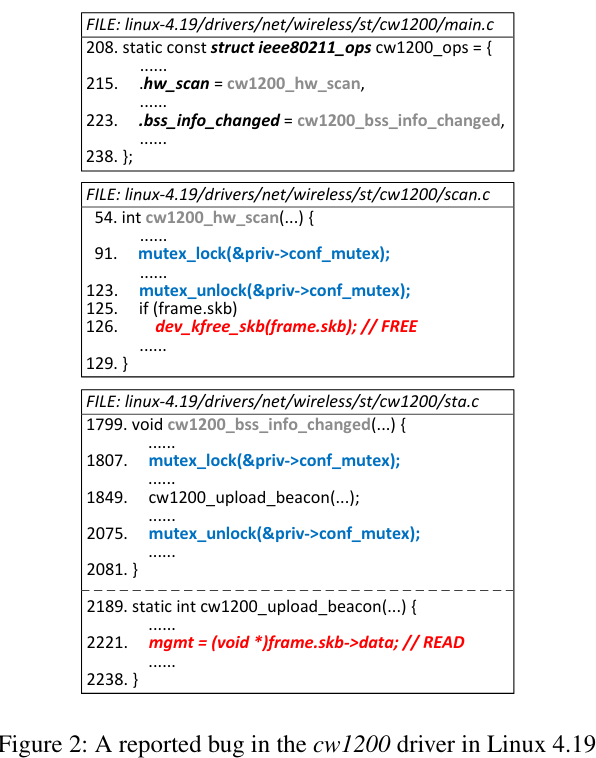
\includegraphics[height=0.9\textheight]{../betterpl/linux-conc-uaf-fig}
};
\node[anchor=north west,font=\small,align=left] at (fig.north east) {
Figure from Bai, Lawall, Chen and Mu \\ (Usenix ATC'19) \\
{\scriptsize ``Effective Static Analysis of Concurrency} \\ {\scriptsize Use-After-Free Bugs in Linux drivers''} \\
~ \\
bug in a wireless networking driver
};
\end{tikzpicture}
\end{frame}


\subsection{concurrency}
\begin{frame}{data races}
    \begin{itemize}
    \item Rusts rules around modification built assuming concurrency
    \item OSes and other ``systems programming'' applications use multiple cores/threads
    \item particular problem: value being used from multiple threads at same time
    \end{itemize}
\end{frame}

\begin{frame}[fragile,label=raceUAF]{data races from use-after-free}
\begin{itemize}
\item given x: Rc<Foo> variable calling x.clone() on two cores
    \begin{itemize}
    \item some variable shared between two cores
    \item reference counting will prevent use-after-free, right?
    \end{itemize}
\end{itemize}
\begin{Verbatim}
x.clone on core A           x.clone on core B
-------------------------------------------
x.inc_strong():
  temp <- self.count
                            x.inc_strong():
                              temp <- self.count
                              self.count <- temp + 1
  self.count <- temp + 1
\end{Verbatim}
\begin{itemize}
\item problem: reference count one too low!
\end{itemize}
\end{frame}

\begin{frame}{Rust solution?}
\begin{itemize}
\item one option: require Rc implementation to handle mutiple cores
    \begin{itemize}
    \item problem: not zero overhead
    \end{itemize}
\item Rust solution: different types for multithreaded/multicore code
\item two ``traits'' to mark custom types:
    \begin{itemize}
    \item Sync: can be used from multiple cores/threads at once
    \item Send: can be moves from one thread to another
    \end{itemize}
\item two implementations of referenc counting
    \begin{itemize}
    \item Rc: not suitable for multicore, not marked Sync/Send
    \item Arc: is suitable for multicore, slower than Rc probably
    \end{itemize}
\end{itemize}
\end{frame}


\section{aside: other language enforcement?}
\begin{frame}{other things languages can enforce?}
    \begin{itemize}
    \item saw: enforcing no use-after-free
    \item lots of coding conventions we might try to enforce:
    \vspace{.5cm}
    \item code's runtime does not depend on secret data
        \begin{itemize}
        \item secret data has different type
        \item variable time operations prohibited with secret data
        \end{itemize}
    \item sensitive data not passed to wrong place
        \begin{itemize}
        \item sensitive data has different type
        \item assignment to wrong places is a type error
        \end{itemize}
    \item code has bounded runtime
        \begin{itemize}
        \item langauge prohibits not unbounded loops, recursion, etc.
        \end{itemize}
    \end{itemize}
\end{frame}


% FIXME: example of concurrency based exploit in Linux

\subsection{other Rust smart pointers}

\begin{frame}{other policies Rust supports}
    \begin{itemize}
        \item \myemph<2>{RefCell} --- borrowing, but check at runtime, not compile-time
            \begin{itemize}
            \item detect at runtime if used while already used
            \item internally: destructor call when returned object goes out of scope
            \end{itemize}
        \item Weak --- reference-counting, but don't contribute to count
            \begin{itemize}
            \item detect at runtime if used with count = 0
            \end{itemize}
        \item Mutex --- with multicore, enforce one user at a time by waiting
        \item \ldots
    \end{itemize}
\end{frame}




\subsection{exercise: smart pointer use case}
\begin{frame}{exercise: which smart pointer?}
    \begin{itemize}
    \item Rc, Arc (reference counting, w/ or w/o threading support
    \item RefCell (borrowing, check at runtime)
    \item Weak (reference counting, but don't contribute to count --- works with Rc)
    \item Mutex (with multicore, one-at-a-time by waiting)
    \vspace{.5cm}
    \item say I have flight reservation system with Flight objects that have
        references to Ticket objects and vice-versa, \\
        and Customer objects that have references to Ticket objects and vice-versa?
    \end{itemize}
\end{frame}


\subsection{Rust linked list}
\begin{frame}[fragile,label=rLL]{Rust linked list}
    \begin{itemize}
    \item not actually a good idea
    \item use \verb|Box<...>| to represent object on the heap
    \item no null, use \verb|Option<Box<...>>| to represent pointer.
    \end{itemize}
\end{frame}

\begin{frame}[fragile,label=rustLL]{Rust linked list (not recommended)}
\begin{minted}[fontsize=\fontsize{9}{10}\selectfont]{Rust}
struct LinkedListNode {
    value: u32,
    next: Option<Box<LinkedListNode>>,
}

fn allocate_list() -> LinkedListNode {
    return LinkedListNode {
        value: 1,
        next: Some(Box::new(LinkedListNode {
            value: 2,
            next: Some(Box::new(LinkedListNode {
                value: 3,
                next: None
            }))
        }))
    }
}
\end{minted}
\end{frame}

\begin{frame}[fragile,label=rustLLNoBox1]{why the box? (1)}
\begin{minted}[fontsize=\fontsize{10}{11}\selectfont]{Rust}
struct LinkedListNode { // ERROR
    value: u32,
    next: Option<LinkedListNode>,
}

// error[E0072]: recursive type `LinkedListNode` has infinite size
\end{minted}
\end{frame}

\begin{frame}[fragile,label=rustLLNoBox2]{why the box? (2)}
\begin{minted}[fontsize=\fontsize{10}{11}\selectfont]{Rust}
struct LinkedListNode { // ERROR
    value: u32,
    next: Option<&LinkedListNode>,
}
// error[E0106]: missing lifetime specifier
//  --> src/main.rs:48:18
//    |
// 48 |     next: Option<&LinkedListNode>,
//    |                  ^ expected lifetime parameter
\end{minted}
\end{frame}


\section{zero-overhead}

\begin{frame}{zero-overhead}
    \begin{itemize}
    \item normal case --- lifetimes --- have no overhead
    \item compiler proves safety, generates code with no bookkeeping
        \vspace{.5cm}
    \item other policies (e.g. reference counting) do
    \item \ldots but can implement new ones if not good enough
    \end{itemize}
\end{frame}



\section{aside: other language enforcement?}
\begin{frame}{other things languages can enforce?}
    \begin{itemize}
    \item saw: enforcing no use-after-free
    \item lots of coding conventions we might try to enforce:
    \vspace{.5cm}
    \item code's runtime does not depend on secret data
        \begin{itemize}
        \item secret data has different type
        \item variable time operations prohibited with secret data
        \end{itemize}
    \item sensitive data not passed to wrong place
        \begin{itemize}
        \item sensitive data has different type
        \item assignment to wrong places is a type error
        \end{itemize}
    \item code has bounded runtime
        \begin{itemize}
        \item langauge prohibits not unbounded loops, recursion, etc.
        \end{itemize}
    \end{itemize}
\end{frame}


\subsection{example: constant time languages}
\begin{frame}{some constant time ideas}
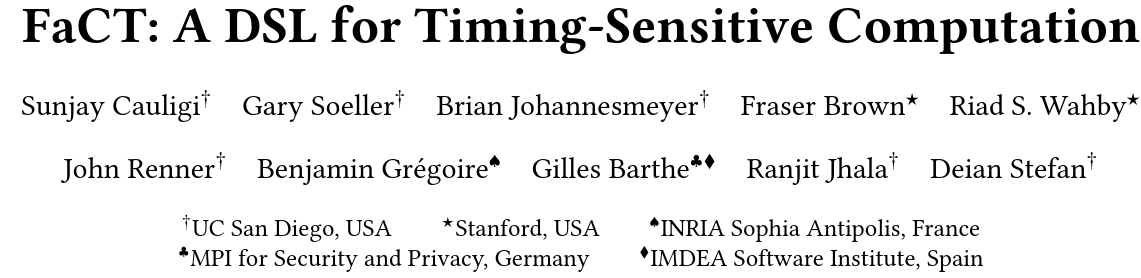
\includegraphics[width=0.8\textwidth]{../betterpl/fact-title}
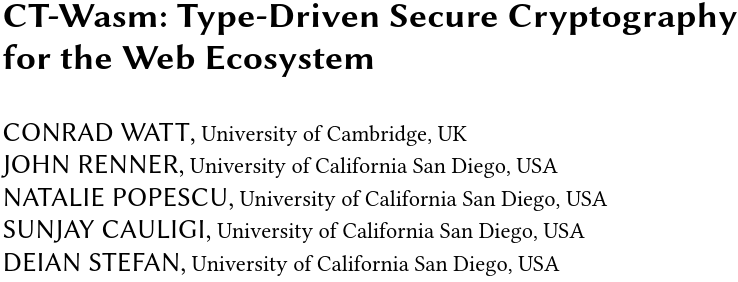
\includegraphics[width=0.8\textwidth]{../betterpl/ct-wasm-title}
\begin{itemize}
\item FaCT, PLDI 2019; CT-Wasm: POPL 2019
\end{itemize}
\end{frame}

\begin{frame}{constant-time programming languages}
    \begin{itemize}
    \item active research area, no consensus on what works best
    \vspace{.5cm}
    \item common approach: separate type for \textbf{secret} data
    \item compiler or language virtual machine disallows variable-time operations using secret data
    \item no secret-based array lookup (cache timing varies)
        \begin{itemize}
        \item e.g. array[secret\_value] $\rightarrow$ compile error (type mismatch)
        \end{itemize}
    \item no secret-based integer division (usually variable speed instruction)
    \item \ldots
    \vspace{.5cm}
    \item explicit operations for any secret-to-non-secret conversions
    \end{itemize}
\end{frame}




\usetikzlibrary{calc}

\section{adding bounds checking}
\begin{frame}{so far}
    \begin{itemize}
    \item many vulnerabilities we looked at due to poor bounds checking
        \begin{itemize}
        \item one exception: use-after-free and related
        \end{itemize}
    \vspace{.5cm}
    \item can we just fix this?
    \end{itemize}
\end{frame}


\subsection{compiler-added?}

\begin{frame}[fragile,label=fortifyMemCpyIntro]{adding bounds checking}
\lstset{language=C,style=small}
\begin{lstlisting}
char buffer[42];
memcpy(buffer, attacker_controlled, len);
\end{lstlisting}
    \begin{itemize}
        \item couldn't compiler add check for \texttt{len}
        \item modern Linux: it does
    \end{itemize}
\end{frame}

\begin{frame}[fragile,label=boundsChecking]{added bounds checking}
\lstset{language=C,style=small}
\begin{lstlisting}
char buffer[42];
memcpy(buffer, attacker_controlled, len);
\end{lstlisting}
\lstset{language=myasm,style=small}
\begin{lstlisting}
    subq   $72, %rsp
    leaq   4(%rsp), %rdi
    movslq len, %rdx
    movq   attacker_controlled, %rsi
    movl   $42, %ecx
    call   __memcpy_chk
\end{lstlisting}
    \begin{itemize}
        \item length \texttt{42} passed to \texttt{\_\_memcpy\_chk}
    \end{itemize}
\end{frame}

\begin{frame}{\_FORTIFY\_SOURCE}
    \begin{itemize}
        \item Linux C standard library + GCC features
        \item adds automatic checking to a bunch of string/array functions
        \item also printf (disable \texttt{\%n} unless format string is a constant)
        \vspace{.5cm}
        \item often enabled by default
        \item GCC options:
            \begin{itemize}
                \item \texttt{-D\_FORTIFY\_SOURCE=1} --- enable (backwards-compatible only)
                \item \texttt{-D\_FORTIFY\_SOURCE=2} --- enable (constant sizes only)
                \item \texttt{-D\_FORTIFY\_SOURCE=3} --- enable (computed sizes, sometimes)
                \item \texttt{-U\_FORTIFY\_SOURCE} --- disable
            \end{itemize}
    \end{itemize}
\end{frame}


\begin{frame}[fragile,label=fortifySrcExample]{bounds checking will happen...}
will add checks (gcc 9.3 \textbf{-O2}, FORTIFY\_SOURCE=1/2)
\begin{lstlisting}[language=C,style=smaller]
void example1() {
    char dest1[1024]; memcpy(dest1, ...); ...
}
char dest2[1024];
void example2() {
    memcpy(dest2, ...); ...
}
void example3() {
    char *p = &dest2[4]; memcpy(p, ...); ...
}
\end{lstlisting}
\end{frame}

\begin{frame}[fragile,label=fortifySrcExample2]{bounds checking will happen...}
will add checks (gcc 14.2 or clang 20 \textbf{-Os}, FORTIFY\_SOURCE=3)
\begin{lstlisting}[language=C,style=smaller]
char dest2[1024];
void example4() {
    char *p = &dest2[mystery()]; memcpy(p, ...); ...
}
\end{lstlisting}
\begin{itemize}
\item no checking with FORTIFY\_SOURCE=2
\item extra overhead: computing min(50, 1024-mystery())
\end{itemize}
\end{frame}

\begin{frame}[fragile,label=fortifySrcExample3]{bounds checking will happen...}
will add check (gcc 14.2 or clang 20 \textbf{-Os}, FORTIFY\_SOURCE=3)
\begin{lstlisting}[language=C,style=smaller]
char dest2[1024];
void example5() {
    char dest3[128];
    char *p = dest2;
    if (mystery()) p = dest3;
    memcpy(p, ...); ...
}
\end{lstlisting}
\begin{itemize}
\item checks for maximum possible with FORTIFY\_SOURCE=2
\end{itemize}
\end{frame}

\begin{frame}[fragile,label=fortifySourceExample4]{bounds checking won't happen...}
\begin{lstlisting}[language=C,style=smaller]
char dest2[1024];
struct Foo {
    char buffer1[128];
    int *pointer;
    ...
};
void example6(struct Foo *f, int size) {
    memcpy(f->buffer1, dest2, size);
}
\end{lstlisting}
\end{frame}

\begin{frame}[fragile,label=fortifySourceExample4]{bounds checking won't quite happen...}
\begin{lstlisting}[language=C,style=smaller]
char dest2[1024];
struct Foo {
    char buffer1[128];
    int *pointer;
    ...
};
struct Foo f;
void example6(int size) {
    memcpy(f.buffer1, dest2, size);
}
\end{lstlisting}
\begin{itemize}
\item checks that size is less than sizeof(struct Foo) (not 128)
\end{itemize}
\end{frame}

\begin{frame}{implementation}
    \begin{itemize}
    \item GCC/clang expose `object size` and `dynamic object size' function
    \item relies on compiler analysis to know size from see declaration or malloc/etc. assignemnt
    \vspace{.5cm}
    \item limited
    \end{itemize}
\end{frame}

\subsection{and library functions}
        % FIXME: exercise: what should call have been
            % needs answers

\begin{frame}[fragile,label=nonChecking]{non-checking library functions}
\lstset{language=C,style=small}
    \begin{itemize}
    \item some C library functions make bounds checking hard: 
\begin{lstlisting}
strcpy(dest, source);
strcat(dest, source);
sprintf(dest, format, ...);
\end{lstlisting}
    \item bounds-checking versions (\myemph{added to library later}):
\begin{lstlisting}
/* might not add \0 (!) */
strncpy(dest, source, size);
strncat(dest, source, size);
snprintf(dest, size, format, ...);
\end{lstlisting}
    \end{itemize}
\end{frame}

\begin{frame}[fragile,label=poorBoundsChecking]{poor bounds-checking APIs}
\begin{lstlisting}[language=C,style=smaller]
char dest[100];
/* THIS CODE IS BROKEN */
strncpy(dest, source1, sizeof dest);
strncat(dest, source2, sizeof dest);
printf("result was %s\n", dest)
\end{lstlisting}
\begin{itemize}
\item the above can access memory of out of bounds
\item \ldots in a bunch of ways
\end{itemize}
\end{frame}

\begin{frame}[fragile,label=strncpyManual]{Linux's strncpy manual}
\begin{lstlisting}[language=C,style=smaller]
strncpy(dest, source1, sizeof dest);
\end{lstlisting}
\begin{itemize}
\item ``Warning: If there is no
       null byte among the first n bytes of src, the string placed in dest will not be null-terminated.''
\end{itemize}
\begin{itemize}
\item exercise: what should the call have been?
\end{itemize}
\end{frame}


\begin{frame}[fragile,label=strncatManual]{Linux's strncat manual}
\begin{lstlisting}[language=C,style=smaller]
strncat(dest, source2, sizeof dest);
\end{lstlisting}
\begin{itemize}
\item ``If src contains n or more bytes, strncat() writes n+1 bytes to  dest  (n
from  src  plus the terminating null byte).  Therefore, the size of dest
must be at least strlen(dest)+n+1.''
\end{itemize}
\begin{itemize}
\item exercise: what should the call have been?
\end{itemize}
\end{frame}

\begin{frame}[fragile,label=betterStrX]{better versions?}
\begin{itemize}
\item FreeBSD (and Linux via libbsd): strlcpy, strlcat
\item ``Unlike [strncat and strncpy], strlcpy() and strlcat() take the full size of the buffer
        and gaurenteeto NUL-terminate the result...''
\end{itemize}
\begin{lstlisting}[language=C++,style=smaller]
strlcpy(dest, source1, sizeof dest);
strlcat(dest, source2, sizeof dest);
\end{lstlisting}
\vspace{.5cm}
\begin{itemize}
\item Windows: \texttt{strcpy\_s}, \texttt{strcat\_s} (same idea, differentname)
\end{itemize}
\end{frame}

\begin{frame}[fragile,label=cppBounds]{C++/Rust bounds checking}
\lstset{language=C,style=small}
\begin{lstlisting}
#include <vector>
...
std::vector<int> data;
data.resize(50);
// undefined behavior:
data[60] = 0;
// throws std::out_of_range exception
data.at(60) = 0;
\end{lstlisting}
\vspace{-\baselineskip}
\hrulefill
\begin{Verbatim}[fontsize=\small]
let data: Vec<i32> = ...;
data.resize(50, 0);
// undefined behavior:
unsafe { *data.get_unchecked_mut(60) = 1; }
// panics at runtime:
data[60] = 0;  
\end{Verbatim}
\end{frame}



\subsection{language support?}


\begin{frame}{language-level solutions}
    \begin{itemize}
    \item languages like Python don't have this problem
    \item couldn't we do the same thing in C?
    \end{itemize}
\end{frame}




\subsection{simple case for bounds checking in C}
\begin{frame}{bounds-checking C}
    \begin{itemize}
    \item there have been many proposals to add bounds-checking to C
    \item including implementations
    \item brainstorm: \myemph{why hasn't this happened?}
    \end{itemize}
\end{frame}

\begin{frame}[fragile,label=addBounds]{easy bounds-checking}
    \lstset{language=C,style=smaller}
\begin{lstlisting}
void vulnerable() {
    char buffer[100];
    int c;
    int i = 0;
    while ((c = getchar()) != EOF && c != '\n') {
        buffer[i] = c;
    }
}
void vulnerable_checked() {
    char buffer[100];
    int c;
    int i = 0;
    while ((c = getchar()) != EOF && c != '\n') {
        FAIL_IF(i >= 100 || i < 0);
        buffer[i] = c;
    }
}
\end{lstlisting}
\end{frame}


\subsection{the problematic case}
\begin{frame}[fragile,label=addBoundsHarder]{harder bounds-checking}
    \lstset{language=C,style=smaller}
\begin{lstlisting}
void vulnerable(char *buffer) {
    char buffer[100];
    int c;
    int i = 0;
    while ((c = getchar()) != EOF && c != '\n') {
        buffer[i] = c;
    }
}
void vulnerable_checked(char *buffer) {
    int c;
    int i = 0;
    while ((c = getchar()) != EOF && c != '\n') {
        FAIL_IF(i >= UNKNOWN || i < UNKNOWN);
        buffer[i] = c;
    }
}
\end{lstlisting}
\end{frame}


\subsection{fat pointer idea}
% FIXME: smoother transition
    % FIXME: exercise about problematic cases


\begin{frame}[fragile,label=wrappedPointers]{adding bounds-checking --- fat pointers}
\lstset{
    language=C,
    style=small
}
\begin{lstlisting}
struct MyPtr {
    char *pointer; /* "raw" pointer value */
    char *minimum; /* first byte of buffer pointed to */
    char *maximum; /* last byte of buffer pointed to */
};
\end{lstlisting}
\begin{visibleenv}<2->
\hrule
\begin{lstlisting}
char buffer[100];
char *p = &buffer[10];
\end{lstlisting}
becomes
\begin{lstlisting}
char buffer[100];
MyPtr p = {
    .pointer = &buffer[10],
    .minimum = &buffer[0],
    .maximum = &buffer[99]
};
\end{lstlisting}
\end{visibleenv}
\end{frame}



\subsubsection{strcpy example}
\begin{frame}[fragile,label=wrappedPtrStrcpy]{adding bounds checking --- strcpy}
\lstset{
    language=C,
    style=small
}
\begin{lstlisting}
MyPtr strcpy(MyPtr dest, const MyPtr src) {
    int i;
    do {
        CHECK(src.pointer + i <= src.maximum);
        CHECK(src.pointer + i >= src.minimum);
        CHECK(dest.pointer + i <= dest.maximum);
        CHECK(dest.pointer + i >= dest.minimum);
        dest.pointer[i] = src.pointer[i];
        i += 1;
        CHECK(src.pointer + i <= src.maximum);
        CHECK(src.pointer + i >= src.minimum);
    } while (src.pointer[i] != '\0');
    return dest;
}
\end{lstlisting}
\end{frame}




\subsubsection{overhead?}

\begin{frame}{speed of bounds checking}
    \begin{itemize}
    \item two comparisons for every pointer access?
    \item three times as much space for every pointer?
    \end{itemize}
\end{frame}



\subsection{unfortunate things C programmers do}
\begin{frame}[fragile,label=unfortunateCProg1]{unfortunate things C programmers do (1)}
from FreeBSD's bootpd (server for machines that boot from the network):
\begin{lstlisting}[language=C,style=smaller]
struct shared_string {
    unsigned int linkcount;
    char         string[1]; /* Dynamically extended */
};
...
s = (struct shared_string *) smalloc(
        sizeof(struct shared_string) + length
    );
...
\end{lstlisting}
\end{frame}

\begin{frame}[fragile,label=unfortunateCProg2]{unfortunate things C programmers do (2)}
from perl's source code:
\begin{lstlisting}[language=C,style=small]
sv_setuv(my_pool_sv, PTR2UV(my_poolp));
...
/* later, in another function: */
my_pool_t *my_poolp = INT2PTR(my_pool_t*, SvUV(my_pool_sv));
\end{lstlisting}
\begin{itemize}
\item PTR2UV: pointer to Unsigned int Value
\item INT2PTR: integer to pointer value
\end{itemize}
\end{frame}

\begin{frame}[fragile,label=unfortunateCProg3]{unfortunate things C programmers do (3)}
\begin{lstlisting}[language=C,style=small]
struct SuperClass;
struct SubClass {
    struct SuperClass super;
    ...
}

struct SubClass sub;
struct SuperClass *super = &sub.super;
some_function(super);
...
some_function(struct SuperClass *super) {
    ...
    struct SubClass *sub = (struct SubClass *)super;
    ...
}
\end{lstlisting}
\end{frame}



\subsection{fat pointers in reality?}
\begin{frame}{example: CCured}
\begin{itemize}
\item Necula et al, ``CCured:  Type-Safe Retrofitting of Legacy Code'' (2002)
\vspace{.5cm}
\item extension to C to add fat pointers
\item actually three different types of pointers:   
    \begin{itemize}
    \item SAFE: point to single object (not array) or NULL
    \item SEQUENCE: pointer to array with known bounds (like ``fat'' pointers)
    \item DYNAMIC: extra to handles type-casting
    \end{itemize}
\item \textit{needs source changes} to annotate some pointer usage
    \begin{itemize}
    \item especially to allow library function calls
    \end{itemize}
\item 1-\textbf{2.5x} time overhead
\end{itemize}
\end{frame}


\section{baggy bounds checking}

\begin{frame}{research example (2009)}
    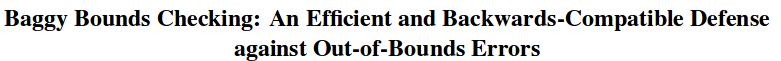
\includegraphics[width=\textwidth]{../bounds/baggy-bounds-title}
\end{frame}

\begin{frame}[fragile,label=lookupTable]{baggy bounds checking idea}
    \begin{itemize}
        \item giant lookup table --- one entry for every 16 bytes of memory
        \item table indicates start of object allocated here
        \item check pointer arithmetic:
    \end{itemize}
\begin{lstlisting}
char p = str[i];
/* becomes: */
CHECK(START_OF[str / 16] == START_OF[&str[i] / 16]);
char p = str[i];
\end{lstlisting}
\end{frame}




\subsection{trick for good performance}

\begin{frame}[fragile,label=baggyBoundsTrick]{baggy bounds trick}
\lstset{language=C,style=small}
    \begin{itemize}
        \item table of pointers to starting locations would be huge
        \item add some restrictions:
            \begin{itemize}
            \item all object sizes are powers of two
            \item all object starting addresses are a multiple of their size
            \end{itemize}
        \item then, table contains size info only:
            \begin{itemize}
            \item table contains $i$, size is $2^i$ bytes:
            \end{itemize}
    \end{itemize}
\begin{lstlisting}
char *GetStartOfObject(char *pointer) {
    return pointer & ~(1 << TABLE[pointer / 16] - 1);
    /* pointer bitwise-and 2^(table entry) - 1 */
    /* clear lower (table entry) bits  of pointer */
}
\end{lstlisting}
\end{frame}



\subsection{the lookup table}
\usetikzlibrary{fit,matrix}

\tikzset{
    stackBox/.style={very thick},
    allocBox/.style={dashed,very thick,fill=blue!20},
    onStack/.style={thick},
    frameOne/.style={fill=blue!15},
    frameTwo/.style={fill=red!15},
    markLine/.style={blue!50!black},
    markLineB/.style={red!90!black},
    hiLine/.style={red!90!black},
}
\begin{frame}<1-6>[fragile,label=lkpTble]{allocations and lookup table}
    \begin{tikzpicture}
        \draw[onStack] (0, 0) rectangle (4, -7);
        \draw[allocBox] (0, 0) rectangle (4, -0.4);
        \draw[stackBox] (0, 0) rectangle (4, -0.5);
        \draw[allocBox] (0, -0.5) rectangle (4, -0.8);
        \draw[stackBox] (0, -0.5) rectangle (4, -1.0);
        \draw[allocBox] (0, -1) rectangle (4, -1.9);
        \draw[stackBox] (0, -1) rectangle (4, -2);
        \draw[allocBox] (0, -2) rectangle (4, -2.4);
        \draw[stackBox] (0, -2) rectangle (4, -2.5);
        \draw[allocBox] (0, -2.5) rectangle (4, -2.7);
        \draw[stackBox] (0, -2.5) rectangle (4, -3);
        \draw[stackBox] (0, -3) rectangle (4, -4);
        \draw[allocBox] (0, -4) rectangle (4, -5.2);
        \draw[stackBox] (0, -4) rectangle (4, -6);

        \begin{visibleenv}<1->
            \node[anchor=north west,align=left] at (9, 0) {
                object allocated in \\ \myemph<1>{power-of-two `slots'}
            };
        \end{visibleenv}
        \begin{visibleenv}<2->
            \matrix[tight matrix,
                nodes={text width=1cm,font=\small\tt},anchor=north west,label={north:table}] (tbl) at (7, -1) {
                $2^4$ \\ $2^4$  \\ $2^5$ \\ $2^5$ \\ $2^4$ \\ $2^4$ \\
                $0$ \\ $0$ \\
                $2^6$ \\ $2^6$ \\ $2^6$ \\ $2^6$ \\
            };
            \begin{scope}[thick,dotted,-Latex]
            \draw (4, -.25) -- (tbl-1-1.west);
            \draw (4, -.75) -- (tbl-2-1.west);
            \draw (4, -1.25) -- (tbl-3-1.west);
            \draw (4, -1.75) -- (tbl-4-1.west);
            \draw (4, -2.25) -- (tbl-5-1.west);
            \draw (4, -2.75) -- (tbl-6-1.west);
            \draw (4, -3.25) -- (tbl-7-1.west);
            \draw (4, -3.75) -- (tbl-8-1.west);
            \draw (4, -4.25) -- (tbl-9-1.west);
            \end{scope}
        \end{visibleenv}
        \begin{visibleenv}<3>
            \draw[ultra thick,red] (0, -1) rectangle (4, -2);
            \node[draw,ultra thick,red,inner sep=0mm,fit=(tbl-3-1) (tbl-4-1)] {};
            \draw[ultra thick,blue] (0, -4) rectangle (4, -6);
            \node[draw,ultra thick,blue,inner sep=0mm,fit=(tbl-9-1) (tbl-12-1)] {};
        \end{visibleenv}
        \begin{visibleenv}<3->
            \node[anchor=north west,align=left] at (9, -2) {
                table stores sizes \\
                \myemph{for each 16 bytes}
            };
        \end{visibleenv}
        \begin{visibleenv}<4>
            \draw[ultra thick,red] (0, -3) rectangle (4, -4);
            \node[draw,ultra thick,red,inner sep=0mm,fit=(tbl-7-1) (tbl-8-1)] {};
        \end{visibleenv}
        \begin{visibleenv}<4->
            \node[anchor=north west,align=left] at (9, -3.5) {
                addresses \textbf<4>{multiples of size} \\
                (may \myemph{require padding})
            };
        \end{visibleenv}
        \begin{pgfonlayer}{bg}
        \begin{visibleenv}<5>
            \fill[red!30] (0, -5.2) rectangle (4, -6.);
            \fill[red!30] (0, -2.7) rectangle (4, -3.);
            \fill[red!30] (0, -1.9) rectangle (4, -2.);
            \fill[red!30] (0, -2.4) rectangle (4, -2.5);
            \fill[red!30] (0, -0.8) rectangle (4, -1.);
            \fill[red!30] (0, -0.4) rectangle (4, -0.5);
        \end{visibleenv}
        \end{pgfonlayer}
        \begin{visibleenv}<5->
            \node[anchor=north west,align=left] at (9, -5.5) {
                sizes are \textbf<5>{powers of two} \\
                (may \myemph{require padding})
            };
        \end{visibleenv}
    \end{tikzpicture}
\end{frame}

\begin{frame}[fragile,label=managing]{managing the table}
    \begin{itemize}
        \item not just done \texttt{malloc()/new}
        \item also for stack allocations:
    \end{itemize}
    \begin{lstlisting}[style=small,language=C]
void vulnerable() {
    char buffer[100];
    gets(vulnerable);
}
\end{lstlisting}
    \begin{tikzpicture}[remember picture, overlay]
        \node[anchor=north east] at ([xshift=-.25cm, yshift=-1cm]current page.north east) {
    \begin{lstlisting}[style=small,language=myasm]
vulnerable:
  // make %rsp a multiple
  // of 128 (2^7) 
  andq $0xFFFFFFFFFFFFFF80, %rsp
  // allocate 128 bytes
  subq $0x80, %rsp
  // rax <- rsp / 16
  movq $rsp, %rax
  shrq $4, %rax
  movb $7, TABLE(%rax)
  movb $7, TABLE+1(%rax)
  ...
  movq %rsp, %rdi
  call gets
  ret
\end{lstlisting}
};
    \end{tikzpicture}
\end{frame}

\begin{frame}[fragile,label=sparseLookup]{sparse lookup table}
    \begin{tikzpicture}
        \node[anchor=south] at (3.5, 3) {lookup table};
        \draw[stackBox] (0, 3) rectangle (7, -3);
        \draw[pattern color=red,pattern=north west lines,onStack] (0, -3) rectangle (7, -1.5)
            node[midway,fill=white,align=center] {unallocated memory (segfault) };
        \draw[fill=green,onStack] (0, -1.5) rectangle (7, .2)
            node[midway] { allocated part of table };
        \draw[pattern color=red,pattern=north west lines,onStack] (0, .20) rectangle (7, 1.3)
            node[midway,fill=white,align=center] {unallocated memory (segfault) };
        \draw[fill=green,onStack] (0, 1.3) rectangle (7, 1.6);
        \draw[pattern color=red,pattern=north west lines,onStack] (0, 1.6) rectangle (7, 2.3);
        \draw[fill=green,onStack] (0, 2.3) rectangle (7, 3)
            node[midway] { allocated part of table };
    \end{tikzpicture}
\end{frame}



\subsection{checks using table}
\usetikzlibrary{calc}
\begin{frame}{baggy bounds check: added code}
    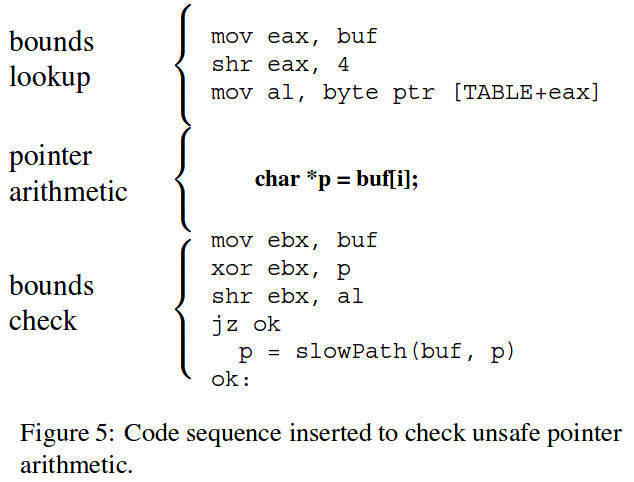
\includegraphics[width=0.6\textwidth]{../bounds/bb-bounds-check}
\end{frame}

\begin{frame}[fragile,label=addedCode]{baggy bounds check: added code}
    \lstset{language=myasm,style=small}
    \begin{lstlisting}
/* bounds lookup */
    mov buf, %rax
    shr %rax, 4
    mov LOOKUP_TABLE(%rax), %al
/* array element address computation */
    ...    // `\textbf{\textit{char * p = buf[i];}}`
/* bound check */
    mov buf, %rbx
    xor p, %rbx
    shr %al, %rbx
    jz  ok
    ...    // handle possible violation
ok:
\end{lstlisting}

    \imagecredit{adapted from paper figure}
\end{frame}

\begin{frame}{avoiding checks}
    \begin{itemize}
        \item code not added if not array/pointer accesses to object
        \item code not added when pointer accesses ``obviously'' safe
            \begin{itemize}
            \item author's implementation: only checked within function
            \end{itemize}
    \end{itemize}
\end{frame}



\subsection{exercise: overhead estimating?}
\begin{frame}<1>[fragile,label=bbOverheadExer1]{exercise: overhead of baggy bounds (1)}
\begin{itemize}
\item suppose program allocates:
    \begin{itemize}
    \item 1000 100 byte objects
    \item 1 10000 byte object
    \end{itemize}
\item using baggy bounds, estimate:
    \begin{itemize}
    \item space required for padding
        \begin{itemize}
        \item<2-> $(128-100)\cdot 1000 + (16384 - 10000)) = 34384$
        \end{itemize}
    \item space required for table
        \begin{itemize}
        \item<2-> $(128\cdot 1000 + 16384) \div 16 = 9024$
        \end{itemize}
    \end{itemize}
\end{itemize}
\end{frame}

\iftoggle{heldback}{}{\againframe<2>{bbOverheadExer1}}

\begin{frame}[fragile,label=bbOverheadExer2]{exercise: overhead of baggy bounds (2)}
\begin{lstlisting}[language=C,style=smaller]
char *strcat(char *d, char *s) {
    int i;
    for (i = 0; s[i] != '\0'; i += 1) {
        d[i] = s[i]; 
    }
    d[i] = '\0';
    return d;
}
\end{lstlisting}
\begin{itemize}
\item estimate:
\begin{itemize}
\item number of bounds checks needed
\item very rough number of instructions run w/o bounds check
\end{itemize}
\item thought question: \\
with bounds checking, what's fastest possible code?
\end{itemize}
\end{frame}


\subsection{alternative: pointer tagging}

\begin{frame}{alternate approach: pointer tagging}
    \begin{itemize}
        \item some bits of \myemph{address} are size 
        \begin{itemize}
        \item replaces table entry/lookup
        \end{itemize}
    \item change code to allocate objects this way
    \item works well on 64-bit --- plenty of addresses to use
    \end{itemize}
    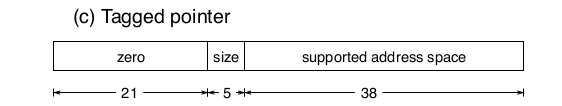
\includegraphics[width=0.8\textwidth]{../bounds/baggy-bounds-tagging}
\end{frame}



\subsection{performance?}

\begin{frame}{baggy bounds performance}
    \begin{itemize}
        \item table: 4--72\% time overhead (depends on benchmark suite)
        \item table: 11--21\% space overhead (depends on benchmark suite)
        \item tagged pointers: slightly better on average
    \end{itemize}
\end{frame}

\begin{frame}{baggy bounds performance}
    \begin{center}
    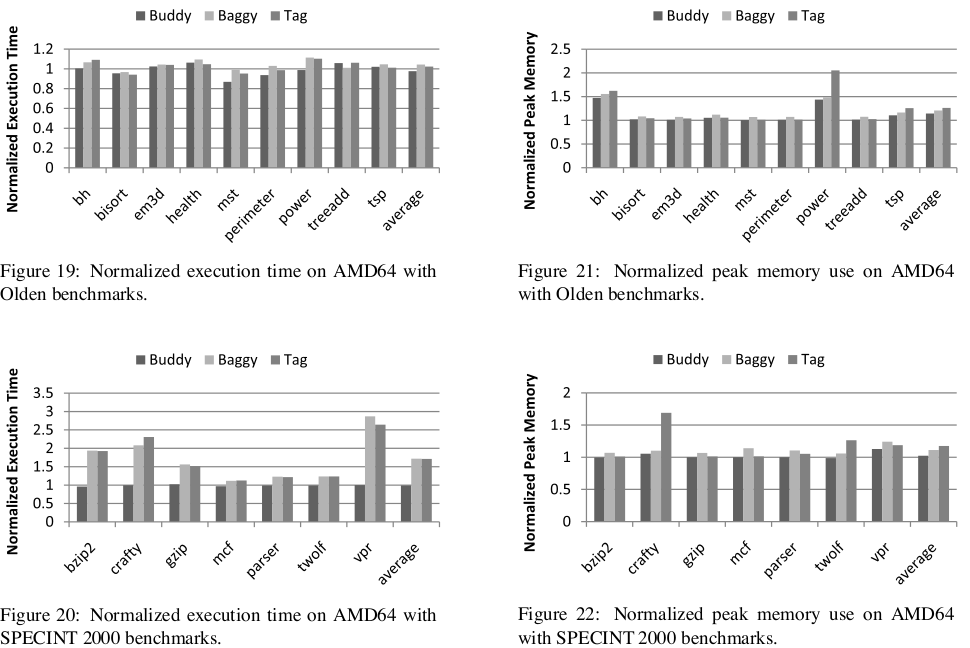
\includegraphics[height=0.8\textheight]{../bounds/baggy-bounds-perf}
    \end{center}
\end{frame}



\subsection{problem: pointers within objects}
% FIXME
\begin{frame}[fragile,label=withinObj]{problem: within object}
\begin{lstlisting}
struct foo {
    char buffer[1024];
    int *pointer;
};
struct foo array_of_foos[1024];
...
char *p = &array_of_foos[4].buffer[4]
\end{lstlisting}
\begin{itemize}
\item exercise: what are the bounds for p?
\end{itemize}
\end{frame}


\subsection{corner cases}

\begin{frame}[fragile,label=unfortunateCProgF2C]{unfortunate things C programmers do (4)}
in code generated by f2c (Fortran to C translator) \\
{\scriptsize (cleaned up slightly)}
\begin{lstlisting}[language=C,style=small]
float sum(int size, float *arr) {
    arr = arr - 1; /* <-- deliberately out-of-bounds pointer */
    float result = 0.f;
    for (i = 1; i <= size; ++i) {
        result += arr[i]
    }
    return result;
}
\end{lstlisting}
\end{frame}



\section{AddressSanitizer}

\begin{frame}{AddressSanitizer}
    \begin{itemize}
    \item like baggy bounds:
        \begin{itemize}
        \item big lookup table
        \item lookup table set by memory allocations
        \item compiler modification: change stack allocations
        \end{itemize}
    \item unlike baggy bounds:
        \begin{itemize}
        \item check reads/writes (instead of pointer computations)
        \item only detect errors that read/write \myemph{between objects}
        \item object sizes not padded to power of two
        \item table has info for every single byte (more precise)
        \end{itemize}
    \end{itemize}
\end{frame}




\subsection{ASan's added check}

\begin{frame}[fragile,label=asanVBounds]{adding bounds-checking example}
\lstset{
    language=C++,
    style=small,
    moredelim={**[is][\btHL<2>]{~2~}{~end~}},
}
\begin{lstlisting}
void vulnerable(long value, int offset) {
    long array[10] = {1,2,3,4,5,6,7,8,9,10};
    // generated code: (added by AddressSanitizer)
    ~2~if (!lookup_table[&array[offset]] == VALID) FAIL();~end~
    array[offset] = value;
    do_something_with(array);
}
\end{lstlisting}
    \begin{itemize}
        \item AddressSanitizer: crashes only if \lstinline|array[offset]| isn't part of any object
            \begin{itemize}
            \item but no extra space --- single-byte precision
            \end{itemize}
    \end{itemize}
\end{frame}



\subsection{stack layout}
\usetikzlibrary{arrows.meta,matrix,patterns}
\tikzset{
    stackBox/.style={very thick},
    allocBox/.style={dashed,very thick,fill=blue!20},
    onStack/.style={thick},
    frameOne/.style={fill=blue!15},
    frameTwo/.style={fill=red!15},
    markLine/.style={blue!50!black},
    markLineB/.style={red!90!black},
    hiLine/.style={red!90!black},
}
\begin{frame}[fragile,label=asanStackLayout]{AddressSanitizer stack layout}
    \begin{tikzpicture}
        \begin{scope}[x=1.7cm]
    \draw[stackBox] (0, 0) rectangle (5, -6);
            \draw[onStack] (0, 0) rectangle (5, -.5)
        node[midway] (arrayLoc) { return address (for \texttt{vulernable()}) };
    \begin{visibleenv}<2>
        \node[anchor=west] at (5.25, -.25) { $\approx$ \tt array[0x13]};
        \node[anchor=west] at (5.25, -3.75) { $\approx$ \tt array[0xa]};
    \end{visibleenv}
    \draw[onStack] (0, -.5) rectangle (5, -1)
        node[midway] { saved \tt\%rbp };
    \draw[onStack] (0, -1) rectangle (5, -1.5)
        node[midway] { saved \tt\%r13 };
    \draw[onStack] (0, -1.5) rectangle (5, -2)
        node[midway] { saved \tt\%r12 };
    \draw[onStack] (0, -2) rectangle (5, -2.5)
        node[midway] { saved \tt\%rbx };
    \draw[onStack,pattern=north west lines,pattern color=red] (0, -2.5) rectangle (5, -4)
        node[midway,fill=white] { ``red zone'' };
    \draw[onStack] (0, -4) rectangle (5, -6)
        node[midway,fill=white] { \tt array };
            \draw[onStack,dashed] (0, -4) rectangle (5, -4.5) node[midway] {\tt array[9]};
            \begin{visibleenv}<3>
            \matrix[tight matrix,
                nodes={text width=3cm,font=\small\tt},anchor=north west,label={north:lookup table}] (tbl) at (6, -2) {
                valid \\ valid  \\ valid \\ valid \\ valid \\ invalid \\ invalid \\
                invalid \\ invalid \\ valid \\ valid \\ \ldots \\
            };
                \draw[thick,-Latex] (5, -.25) -- (tbl-1-1.west);
                \draw[thick,-Latex] (5, -.75) -- (tbl-2-1.west);
            \end{visibleenv}
    \draw[thick,-Latex] (5.15, -6) --++ (0, 2);
        \end{scope}
    \end{tikzpicture}
\end{frame}





\section{AddressSanitizer}

\begin{frame}{AddressSanitizer}
    \begin{itemize}
    \item like baggy bounds:
        \begin{itemize}
        \item big lookup table
        \item lookup table set by memory allocations
        \item compiler modification: change stack allocations
        \end{itemize}
    \item unlike baggy bounds:
        \begin{itemize}
        \item check reads/writes (instead of pointer computations)
        \item only detect errors that read/write \myemph{between objects}
        \item object sizes not padded to power of two
        \item table has info for every single byte (more precise)
        \end{itemize}
    \end{itemize}
\end{frame}




\subsection{ASan's added check}

\begin{frame}[fragile,label=asanVBounds]{adding bounds-checking example}
\lstset{
    language=C++,
    style=small,
    moredelim={**[is][\btHL<2>]{~2~}{~end~}},
}
\begin{lstlisting}
void vulnerable(long value, int offset) {
    long array[10] = {1,2,3,4,5,6,7,8,9,10};
    // generated code: (added by AddressSanitizer)
    ~2~if (!lookup_table[&array[offset]] == VALID) FAIL();~end~
    array[offset] = value;
    do_something_with(array);
}
\end{lstlisting}
    \begin{itemize}
        \item AddressSanitizer: crashes only if \lstinline|array[offset]| isn't part of any object
            \begin{itemize}
            \item but no extra space --- single-byte precision
            \end{itemize}
    \end{itemize}
\end{frame}



\subsection{stack layout}
\usetikzlibrary{arrows.meta,matrix,patterns}
\tikzset{
    stackBox/.style={very thick},
    allocBox/.style={dashed,very thick,fill=blue!20},
    onStack/.style={thick},
    frameOne/.style={fill=blue!15},
    frameTwo/.style={fill=red!15},
    markLine/.style={blue!50!black},
    markLineB/.style={red!90!black},
    hiLine/.style={red!90!black},
}
\begin{frame}[fragile,label=asanStackLayout]{AddressSanitizer stack layout}
    \begin{tikzpicture}
        \begin{scope}[x=1.7cm]
    \draw[stackBox] (0, 0) rectangle (5, -6);
            \draw[onStack] (0, 0) rectangle (5, -.5)
        node[midway] (arrayLoc) { return address (for \texttt{vulernable()}) };
    \begin{visibleenv}<2>
        \node[anchor=west] at (5.25, -.25) { $\approx$ \tt array[0x13]};
        \node[anchor=west] at (5.25, -3.75) { $\approx$ \tt array[0xa]};
    \end{visibleenv}
    \draw[onStack] (0, -.5) rectangle (5, -1)
        node[midway] { saved \tt\%rbp };
    \draw[onStack] (0, -1) rectangle (5, -1.5)
        node[midway] { saved \tt\%r13 };
    \draw[onStack] (0, -1.5) rectangle (5, -2)
        node[midway] { saved \tt\%r12 };
    \draw[onStack] (0, -2) rectangle (5, -2.5)
        node[midway] { saved \tt\%rbx };
    \draw[onStack,pattern=north west lines,pattern color=red] (0, -2.5) rectangle (5, -4)
        node[midway,fill=white] { ``red zone'' };
    \draw[onStack] (0, -4) rectangle (5, -6)
        node[midway,fill=white] { \tt array };
            \draw[onStack,dashed] (0, -4) rectangle (5, -4.5) node[midway] {\tt array[9]};
            \begin{visibleenv}<3>
            \matrix[tight matrix,
                nodes={text width=3cm,font=\small\tt},anchor=north west,label={north:lookup table}] (tbl) at (6, -2) {
                valid \\ valid  \\ valid \\ valid \\ valid \\ invalid \\ invalid \\
                invalid \\ invalid \\ valid \\ valid \\ \ldots \\
            };
                \draw[thick,-Latex] (5, -.25) -- (tbl-1-1.west);
                \draw[thick,-Latex] (5, -.75) -- (tbl-2-1.west);
            \end{visibleenv}
    \draw[thick,-Latex] (5.15, -6) --++ (0, 2);
        \end{scope}
    \end{tikzpicture}
\end{frame}



\subsection{can't change object layout?}
\begin{frame}[fragile,label=withinObj]{revisted: within object}
\begin{lstlisting}
struct foo {
    char buffer[1024];
    int *pointer;
};
struct foo array_of_foos[1024];
...
char *p = &array_of_foos[4].buffer[4]
\end{lstlisting}
\begin{itemize}
\item exercise: What out-of-bounds accesses to `p' can AddressSanitizer detect?
\item how does that compare to baggy bounds? To the `fat pointers' strategy?
\end{itemize}
\end{frame}

\usetikzlibrary{arrows.meta,patterns,shapes.misc}
\tikzset{
    stackBox/.style={very thick},
    allocBox/.style={dashed,very thick,fill=blue!20},
    on stack/.style={thick},
    frameOne/.style={fill=blue!15},
    frameTwo/.style={fill=red!15},
    markLine/.style={blue!50!black},
    markLineB/.style={red!90!black},
    hiLine/.style={red!90!black},
}

\begin{frame}[fragile,label=changeObjLayout]{changing object layout?}
\begin{lstlisting}
struct string_list {
    char data[100];
    struct string_list *prev;
    struct string_list *next;
};
\end{lstlisting}
\begin{tikzpicture}[overlay,remember picture]
\node[anchor=south] at (2.5, 0) {actual layout};
\begin{scope}[shift={(0,0)}]
\draw[on stack] (0, 0) rectangle ++(5, -.5)
    node[midway] {prev};
\draw[on stack] (0, -.5) rectangle ++(5, -.5)
    node[midway] {next};
\draw[on stack] (0, -1) rectangle ++(5, -2)
    node[midway] {data};
\draw[thick,-Latex] (5.25, -3) --++ (0, 1);
\end{scope}
\node[anchor=south] at (9.5, 0) {layout wanted for error-finding};
\begin{scope}[shift={(7,0)}]
\draw[on stack] (0, 0) rectangle ++(5, -.5)
    node[midway] {prev};
\draw[on stack] (0, -.5) rectangle ++(5, -.5)
    node[midway] {next};
\draw[on stack,pattern=north west lines, pattern color=red] (0, -1) rectangle ++(5, -1)
    node[midway] {``red zone''};
\draw[on stack] (0, -2) rectangle ++(5, -2)
    node[midway] {data};
\draw[thick,-Latex] (5.25, -4) --++ (0, 1);
\end{scope}
\begin{visibleenv}<2->
\node[ultra thick,draw,red,cross out,minimum width=5cm,minimum height=4cm] at (9.5, -2) {};
\node[rotate=15,draw,thick,fill=red!10,font=\small,align=center] at (9.5, -3) {
    would break calls to libraries \\
    (unless library also rebuilt)
};
\end{visibleenv}
\end{tikzpicture}
\end{frame}


\subsection{pro/con}

\begin{frame}{AddressSanitizer versus Baggy Bounds}
    \begin{itemize}
    \item pros vs baggy bounds:
        \begin{itemize}
        \item you can actually use it (comes with GCC/Clang)
        \item byte-level precision --- no ``padding'' on objects
        \item detects use-after-free a lot of the time
        \end{itemize}
    \item cons vs baggy bounds:
        \begin{itemize}
        \item doesn't prevent out-of-bounds ``targetted'' accesses
        \item requires extra space between objects
        \item usually slower
        \end{itemize}
    \end{itemize}
\end{frame}



\section{valgrind memcheck, briefly}


\begin{frame}{Valgrind Memcheck}
    \begin{itemize}
    \item similar to AddressSanitizer --- but no compiler modificaitons
    \item instead: is a virtual machine (plus alternate malloc/new implementation)
    \vspace{.5cm}
    \item only (reliably) detects errors on heap
    \item but works on \myemph{unmodified} binaries
    \end{itemize}
\end{frame}




\subsection{aside: binary translation}
% From 20170123
\usetikzlibrary{positioning}

\begin{frame}{binary translation}
    \begin{itemize}
    \item compile assembly to new assembly
    \vspace{1cm}
    \item works without instruction set support
    \item early versions of VMWare on x86 (before x86 added virtualisation support)
    \item can be used to run one platform on another
    \end{itemize}
\end{frame}

\begin{frame}[fragile,label=binTransIdea]{binary translation idea}
\lstset{
    language=myasm,
    style=small,
    morekeywords={movq,addss,subss}
}
\begin{tikzpicture}
\tikzset{
    code/.style={inner sep=0mm,align=left},
    hiOn/.style={alt=#1{rounded corners,fill=green,fill opacity=0.3,text opacity=1.0}{}},
    markOn/.style={alt=#1{rounded corners,draw,thick}{}},
}
\node[code,markOn=<2>,hiOn=<3>] (bb1) {
\begin{lstlisting}
0x40FE00: addq %rax, %rbx
movq 14(%r14,4), %rdx
addss %xmm0, (%rdx)
...
0x40FE3A: jne 0x40F404
\end{lstlisting}
};
\node[right=.25cm of bb1,visible on=<2>,align=left] {
    divide machine code \\
    into \textit{basic blocks} \\
    (= ``straight-line'' code) \\
    (= code till \\ 
    jump/call/etc.)
};
\node[code,right=.25cm of bb1,visible on=<3>] (bb1New) {
generated code: \\
\begin{lstlisting}
// addq %rax, %rbx
movq rax_location, %rdi
movq rbx_location, %rsi
call checked_addq
movq %rax, rax_location
...
// jne 0x40F404
... // get CCs 
je do_jne
movq $0x40FE3F, %rdi
jmp translate_and_run
do_jne:
movq $0x40F404, %rdi
jmp translate_and_run
\end{lstlisting}
};
\node[code,markOn=<2>,anchor=north west] (bb2) at (bb1.south west){
\begin{lstlisting}
subss %xmm0, 4(%rdx)
...
je 0x40F543
\end{lstlisting}
};
\node[code,markOn=<2>,anchor=north west] (bb3) at (bb2.south west){
\begin{lstlisting}
ret
\end{lstlisting}
};
\end{tikzpicture}
\end{frame}

\begin{frame}[fragile,label=binTransIdea2]{a binary translation idea}
    \begin{itemize}
    \item convert whole \textit{basic blocks}
        \begin{itemize}
        \item code upto branch/jump/call
        \end{itemize}
    \item end with call to {\tt translate\_and\_run}
        \begin{itemize}
        \item compute new \myemph{simulated PC} address to pass to call
        \end{itemize}
    \end{itemize}
\end{frame}

\begin{frame}[fragile,label=binTransIdea3]{making binary translation fast}
    \lstset{style=small,language=myasm,morekeywords={movq}}
    \begin{itemize}
    \item cache converted code
        \begin{itemize}
        \item {\tt translate\_and\_run} checks cache first
        \end{itemize}
    \item patch calls to {\tt translate\_and\_run} to refer directly to cached code
    \item do something more clever than \lstinline|movq rax_location, ...|
        \begin{itemize}
        \item map (some) registers to registers, not memory
        \end{itemize}
    \item ends up being ``just-in-time'' compiler
    \end{itemize}
\end{frame}


\begin{frame}{binary translation? really?}
    \begin{itemize}
    \item early VMWare: for instructions without hardware virtualization support
        \begin{itemize}
        \item only needed for little bits of OS code
        \end{itemize}
    \item used by Apple to handle changing CPU designs
    \item Rosetta 2: run Intel on ARM (current)
    \item Rosetta: run Power PC on Intel (2005--2011)
    \item Mac 68k emulator: Run Motorola 680x0 on Power PC (1994--2005)
    \end{itemize}
\end{frame}



\subsection{aside: other binary translation applications}
% FIXME

\section{exericse: which prevents}
\begin{frame}{which scheme prevents\ldots?}
\begin{itemize}
\item which schemes detect or prevent from being harmful\ldots?
    \begin{itemize}
    \item 1. call to assembly code that goes beyond buffer?
    \item 2. allowing attacker to insert 150 bytes in 100 byte buffer on heap?
    \item 3. allowing attacker to insert 120 bytes in 100 byte buffer on stack?
    \item 4. attecker exploiting code that does array[attacker\_index] to overwrite something outside heap array?
    \end{itemize}
\item of:
    \begin{itemize}
    \item A. ``fat pointers'' approach
    \item B. Baggy Bounds checking
    \item C. AddressSanitizer
    \item D. Valgrind Memcheck
    \end{itemize}
\end{itemize}
\end{frame}

\begin{frame}{answer (1)}
\begin{itemize}
\item which schemes detect or prevent from being harmful\ldots?
    \begin{itemize}
    \item 1. call to assembly code that goes beyond buffer?
    \end{itemize}
\item only Valgrind Memcheck handles assembly code
\item other techniques require C compiler to produce different assembly
\end{itemize}
\end{frame}

\begin{frame}{answer (2)}
\begin{itemize}
\item which schemes detect or prevent from being harmful\ldots?
    \begin{itemize}
    \item 2. allowing attacker to insert 150 bytes in 100 byte buffer on heap?
    \end{itemize}
\item schemes:
    \begin{itemize}
    \item A. ``fat pointers'' approach --- yes
    \item B. Baggy Bounds checking ---yes, detect + crash
    \item C. AddressSanitizer --- yes, detect + crash
    \item D. Valgrind Memcheck --- yes, detect + rash
    \end{itemize}
\end{itemize}
\end{frame}

\begin{frame}{answer (3)}
\begin{itemize}
\item which schemes detect or prevent from being harmful\ldots?
    \begin{itemize}
    \item 3. allowing attacker to insert 120 bytes in 100 byte buffer on stack?
    \end{itemize}
\item schemes:
    \begin{itemize}
    \item A. ``fat pointers'' approach --- yes
    \item B. Baggy Bounds checking ---prevent from being harmful / no crash
    \item C. AddressSanitizer --- yes, detect + crash (red zone)
    \item D. Valgrind Memcheck --- no --- no memory to mark invalid
    \end{itemize}
\end{itemize}
\end{frame}

\begin{frame}{answer (3)}
\begin{itemize}
\item which schemes detect or prevent from being harmful\ldots?
    \begin{itemize}
    \item 4. attecker exploiting code that does array[attacker\_index] to overwrite something outside heap array?
    \end{itemize}
\item schemes:
    \begin{itemize}
    \item A. ``fat pointers'' approach --- yes
    \item B. Baggy Bounds checking --- yes
    \item C. AddressSanitizer --- no --- attacher index can find valid memory
    \item D. Valgrind Memcheck --- no --- (same as AddressSanitizer)
    \end{itemize}
\end{itemize}
\end{frame}

% FIXME: exercise
    % which scheme will prevent XXX



\section{backup slides}
\begin{frame}{backup slides}
\end{frame}

\end{document}
